\documentclass[conference,letterpaper,retainorgcmds]{IEEEtran}
\IEEEoverridecommandlockouts
% The preceding line is only needed to identify funding in the first footnote. If that is unneeded, please comment it out.
\usepackage{cite}
\usepackage{amsmath,amssymb,amsfonts}
\usepackage{algorithmic}
\usepackage{graphicx}
\usepackage{textcomp}
\usepackage{enumitem}
\usepackage{xcolor}
\usepackage{todonotes}
\def\BibTeX{{\rm B\kern-.05em{\sc i\kern-.025em b}\kern-.08em
    T\kern-.1667em\lower.7ex\hbox{E}\kern-.125emX}}
   
\usepackage{microtype}
\usepackage[utf8]{inputenc} %
\usepackage{subfigure}
% \usepackage{caption}
% \usepackage{subcaption}
\usepackage{booktabs}
\usepackage{hyperref} %
\usepackage{xspace}
\usepackage{listings}
\usepackage{multirow}
\usepackage{enumitem} %
\usepackage[normalem]{ulem}

\newcommand{\leslie}[2]{{\sout{#1}}{ \color{magenta}#2}}
\newcommand{\carlosstrike}[2]{{\sout{#1}}{ \color{cyan}#2}}
\newcommand{\carlos}[1]{{\color{cyan}#1}}

\renewcommand{\baselinestretch}{0.96}
\setlength{\intextsep}{2pt}
\setlength{\floatsep}{0.5pt}
\setlength{\textfloatsep}{10pt}

\newcommand{\nasbench}{\mbox{NAS-Bench-101}\xspace}
\newcommand{\autosklearn}{\textsf{Auto-Sklearn}\xspace}
\newcommand{\irace}{\textsf{\small irace}\xspace}

\begin{document}

\title{Evaluating anytime performance on {NAS-Bench-101}
% \thanks{Identify applicable funding agency here. If none, delete this.}
}

\author{\IEEEauthorblockN{Carlos Vieira}
\IEEEauthorblockA{\textit{IMD, Universidade Federal}\\
\textit{do Rio Grande do Norte}\\
Natal, RN, Brazil \\
carlosv@ufrn.edu.br}
\and
\IEEEauthorblockN{Leslie {Pérez Cáceres}}
\IEEEauthorblockA{\textit{Escuela de Ingeniería Informática} \\
\textit{Pontificia Universidad Católica de Valparaíso}\\
Valparaíso, Chile \\
leslie.perez@pucv.cl}
\and
\IEEEauthorblockN{Leonardo~C.~T. Bezerra}
\IEEEauthorblockA{\textit{IMD, Universidade Federal}\\
\textit{do Rio Grande do Norte}\\
Natal, RN, Brazil \\
leobezerra@imd.ufrn.br}
}



\maketitle
%%% LESLIE: remove the following line for submission
% \pagestyle{plain}    % -- to make other pages number less.



% \begin{abstract}
% Neural architecture search~(NAS) is a field where computational effort poses a significant challenge, requiring large computing clusters and specialized hardware. Furthermore, the lack of common experimental guidelines often compromises NAS comparison or may \leslie{incur in}{induce} premature conclusions. In a recent work, \nasbench was proposed to help mitigate those factors, providing both a common benchmark and experimental guidelines for its use. In this work, we \leslie{}{discuss the design choices in \nasbench and} propose improvements that increase the potential of \leslie{\nasbench}{the benchmark}.
% First, we bridge NAS and the research on anytime performance, showing how a bi-objective formulation of NAS can improve the insights provided \leslie{}{by \nasbench}. Then, we discuss choices made in the design of the benchmark, namely (i)~the fixed-size encoding, (ii)~the effects of the limited variability available, (iii)~\leslie{assessing}{the assessment of} algorithms only from a TPU time perspective, and; (iv)~the number of repetitions proposed.
% We demonstrate our contributions assessing the best-performing algorithms originally benchmarked on \nasbench and also \irace, one of the best-performing algorithm configurators \leslie{(AC)}{} from the literature. Results indicate that (i)~the anytime performance methodology enriches the insights obtained from the assessment on the original \nasbench; (ii)~algorithm comparison is strongly affected by the design choices discussed, and; (iii)~the performance of SMAC in this benchmark is significantly improved by our alternative setups.
% \end{abstract}

% \begin{IEEEkeywords}
% Neural architecture search, performance assessment, anytime optimization
% \end{IEEEkeywords}

% %!TEX root = ../emo.tex
\section{Introduction}

% \leslie{}{
% I write this to clear up ideas. Topics to be covered regarding \nasbench:
% \begin{itemize}
%     \item Number of repetitions of the techniques
%     \item Feasibility regarding execution time of NAS techniques
%     \item Bi-objective formulation (cost/time) or anytime optimization 
%     \item Stochasticity representation missing in the scenario (repetitions) issue in SMAC (caching)
%     \item Representation of the architecture using variable number of nodes.
% \end{itemize}
% }

Neural architecture search~(NAS) is likely the most promising field in automated machine learning~(AutoML) when the data to be modeled is unstructured. Recent NAS breakthroughs include challenging application domains, such as computer vision and natural language processing~\cite{ReaAggHuaLe2019re,ZopLe2017nas,ZopVasShlLeh2018scalable}. These promising applications have evidenced the need for intelligent approaches to mitigate the significant computational effort required for the experimental campaigns involved in the development of NAS techniques.
The development of representative benchmarks that enable fast and standardized experimentation is thus a need in the NAS field.
NAS-Bench-101~\cite{YinKleChrReaMurHut2019nasbench} is a repository of benchmarked convolutional neural networks for the CIFAR-10~\cite{Krizhevsky2009cifar} dataset that can be used by NAS researchers when evaluating or proposing algorithms. \nasbench enables the evaluation of neural architectures in negligible time, providing NAS developers with a fast test suite, and avoiding the duplication of computational effort when evaluating architectures. Besides reusability, \nasbench is also an effort to standardize NAS performance assessment since comparability between different works in the field is in general limited. 


%\leslie{}{[I think here we should introduce why we need to extend the formulation to also include the computational time.]}

In this work, we analyze the design choices in \nasbench and how these relate to the performance insights provided by the benchmark. We propose to enrich the insights provided by \nasbench in three significant ways. First, we formulate NAS as a bi-objective problem comprising solution quality and computational resources consumed. This anytime formulation~\cite{LopStu2013ejor} extends \nasbench final quality approach to an approach that compares the performance dynamics of algorithms in a Pareto-compliant way. Second, we discuss other experimental design choices that underlie \nasbench such as (i)~fixing the number of vertices, which we believe could restrict the potential of NAS algorithms; (ii)~limiting the variability included in the benchmark, which may lead to a weak representation of a NAS scenario, and; (iii)~assessing NAS algorithms solely based on TPU time, overlooking the overhead of the search process of the algorithms. Finally, we revisit the experimental guidelines suggested by \nasbench; specifically, the large number of repetitions suggested to benchmark NAS algorithms. %\carlos{[change paragraph to mirror text/abstract structure?]}

An experimental assessment of high-performing algorithms complements our theoretical discussion. In more detail, we consider two of the best-performing algorithms identified in the original \nasbench assessment, namely regularized evolution~(RE~\cite{ReaAggHuaLe2019re}) and SMAC~\cite{HutHooLey2011lion}. We also include \irace~\cite{LopDubPerStuBir2016irace} in this assessment, an algorithm configurator known to have state-of-the-art performance on the optimization of algorithm design for solution quality~\cite{BezLopStu2020chapter}. Performing a more reasonable number of repetitions than in the extensive campaign adopted in the original \nasbench assessment, we are able to reproduce the same conclusions obtained from the original final-quality performance analysis of RE and SMAC. Furthermore, results show that the algorithm, number of vertices, variability degree, and stopping criterion are interacting factors, confirming our design choice discussion's relevance. 

Even if the algorithms assessed have been configured for final-quality performance, our anytime assessment using a bi-objective optimization methodology enriches the analysis of \nasbench. Specifically, RE is outperformed by the remaining algorithms in the final-quality analysis, but it outperforms \irace regarding anytime performance. We further inspect differences between algorithms with empirical attainment function~(EAF~\cite{LopPaqStu09emaa}) difference plots and observe that RE and SMAC are incomparable under the original \nasbench setup. % Regarding experimental design choices, results show that algorithm, number of vertices, and variability degree are interacting factors, and that SMAC is able to improve significantly under alternative setups proposed. Finally, we remark that our results with a more reasonable number of repetitions match the results from the extensive campaign adopted in the original \nasbench assessment.\sloppy
Regarding the latter, SMAC consistently outperforms the remaining algorithms both concerning final-quality and anytime performance. We believe these results further support our argument that \nasbench assessment should account for NAS computation time, given that the time required by a SMAC execution is considerably larger compared to the time required by a run of RE or \irace.% \carlos{[do we give these times anywhere, or indicate they'll be present in supp material?]}.

We conclude our work with an analysis of the high-performing architectures selected by the NAS algorithms. Interestingly, some of these do not include pooling layers, even if convolutional layers do not constrain feature map dimensions. We believe this result highlights that a bi-objective performance formulation should be discussed not only at NAS level, but also at model training. Though \nasbench provides temporal snapshots of the training process, only the final accuracy of the models is used when assessing an architecture. Thus, costly architectures may be deemed equivalent to much faster ones, clearly an undesirable behavior.

The remainder of this paper is structured as follows. Section~\ref{sec:background} briefly reviews background concepts related to this work, namely neural architecture search, the most relevant NAS algorithm classes and their performance on \nasbench, and anytime optimization. Next, Section~\ref{sec:guidelines} presents our theoretical discussion, in particular the bi-objective formulation for \nasbench and potential impact of benchmark design choices on both final quality and anytime performance. Section~\ref{sec:results} details the final quality results observed for the selected algorithms with regards to the previously discussed benchmark characteristics. The anytime performance of the selected algorithms is discussed in Section~\ref{sec:anytime}. We then conduct an analysis on high-performing architectures in Section~\ref{sec:configurations}. Last, we conclude and discuss future work in Section~\ref{sec:conclusion}.
% %!TEX root = ../emo.tex
\section{Background}
\label{sec:background}

In this work, we bridge the research on NAS and anytime optimization. For context, we define NAS, its application to computer vision, and the inner works of \nasbench. Next, we detail the most relevant NAS algorithm classes, and discuss their performance on \nasbench. Finally, we review how a bi-objective formulation of optimization problems can model anytime performance.

% \subsection{PROBLEM}
% ADD COMPUTER VISION THINGY

% HERE ABOUT ML HYPER-PARAMETERS + NEURAL ARQUITECTURE SEARCH
\subsection{Neural Architecture Search~(NAS)}
From a high-level perspective, NAS comprises the design and configuration of neural networks~\cite{ElsMetHut2019nas-survey}. In the context of deep learning, NAS is being instrumental to challenging fields such as computer vision~\cite{ReaAggHuaLe2019re,ZopLe2017nas,ZopVasShlLeh2018scalable}. Given the computational
overhead it poses, different mitigation approaches have been considered, such as designing architecture cells that are replicated to become larger networks~\cite{ZopLe2017nas,ZopVasShlLeh2018scalable}. This is the approach followed by \nasbench, a benchmark of convolutional networks for CIFAR-10~\cite{Krizhevsky2009cifar}. Below, we detail the most important characteristics of this benchmark:

\begin{description}[style=unboxed, leftmargin=0px]
\item[Design space.] A cell is modeled as a directed acyclic graph~(DAG), where each node represents a neural network layer~(convolutional or pooling). The cell contains up to five layers (not counting input and output layers). Solutions are encoded as (i)~an adjacency matrix, which defines the topology of the cell, and; (ii)~a node label list, which determines the types of layers that will be employed. 
\item[Architecture evaluation.] Performance metrics are provided for different stopping criteria run on tensor processing unit~(TPU) clusters. Besides TPU time, queries to the API provided training, validation, and test accuracy. Results are sampled from three different seeds for variability.
\end{description}

\subsection{NAS Algorithms and Their Performance on \nasbench}

Three major classes of NAS algorithms can be identified in the literature~\cite{ElsMetHut2019nas-survey}, namely evolutionary algorithms~(EAs), algorithm configurators~(AC), and neural networks. In \cite{YinKleChrReaMurHut2019nasbench}, a set of relevant algorithms from each class were applied and compared on \nasbench. The algorithms were compared using as stopping criterion the total TPU time available for the search process~($10^7s$). In that comparison, multi-fidelity algorithms such as HyperBand~\cite{LiJamSal2018hyperband} could not benefit from the different stopping criteria provided. In turn, regularized evolution~(RE,~\cite{ReaAggHuaLe2019re}) and SMAC~\cite{HutHooLey2011lion} stood out. In the following, we give the details of both RE and SMAC. Next, we describe \irace~\cite{LopDubPerStuBir2016irace}, another relevant AC that we assess in this work.

\begin{description}[style=unboxed, leftmargin=0px]
\item[Regularized evolution] is a ($\mu$,1)-EA proposed for NAS that uses accuracy and aging for mating and environmental selection, respectively. In more detail, at each iteration RE maintains a population of candidate architectures. Best-performing architectures regarding accuracy are more likely to be selected to produce a novel candidate architecture. This is achieved by bit-flip mutation to an arbitrary edge, or by replacing an arbitrary node's label with a different label. The novel candidate architecture replaces the oldest candidate in the current population. In particular, authors argue that this aging-based environmental selection promotes regularization. 

\item[SMAC] is a sequential, model-based algorithm configuration procedure. The configuration process in SMAC starts by performing the evaluation of an initial configuration (e.g. a parameter setting known for its good performance).
Then, it alternates between
(i) building a random forest model to predict configuration
performance; (ii) searching the configuration space for promising configurations using
the model as surrogate for performance assessment,
and; (iii) evaluating the selected configurations on the target problem. 
%The most successful applications of SMAC concern reducing  the runtime of heuristic algorithms.
\end{description}

The good performance obtained by SMAC indicates that out-of-the-box ACs have the potential to be good options for real NAS tasks.
%, and thus these results show that such tasks can be approached by general out-of-the-box procedures like SMAC. 
Yet, real NAS tasks pose an additional challenge regarding the computation time that is required for the configuration process. This aspect is not fully addressed in \nasbench, as the configuration task is assessed for final performance. %[CHECK THIS: not sure this is true!]. 
In a real NAS task, the sequential nature of SMAC can be a drawback. 
%Configurations must be evaluated and then performance data must be provided for model training and following sampling. 
Compared to SMAC, HyperBand~(HB) has the advantage of being fully parallel, but HB applies limited learning on its search process, relying entirely on multi-fidelity. % and thus, its performance is not good. 
Another potentially parallelizable algorithm is RE, given the maturity of  the literature on parallel EAs; yet, its current version is sequential. 
%can be applied in parallel and good areas of the solution space are detected due to the evolutionary operators applied.
In this work, we add to the evaluated methods an AC called \irace. Like RE, \irace can be classified as an EA and thus inherently parallelizable. In addition, \irace adopts a learning approach to detect high performing areas of the configuration space and focus on them, as described in the following.

\begin{description}[style=unboxed, leftmargin=0px]
\item[\irace] is an estimation of distribution algorithm
that implements iterated racing for configuration
evaluation.  The AC alternates
between (i) applying a racing procedure in which a
set of configurations is evaluated on subsets of training instances several times,
and; (ii) updating a set of probability
distributions used to sample a set of new configurations for a novel iteration (race). 
At each race, candidate configurations are initially evaluated on a fixed number of instances.
%times (by default 5).
Once these evaluations are completed, a statistical test (Friedman's or Student's t-test) is applied to eliminate poor performing configurations from the race. 
%The elimination test is applied after all configurations in the race complete a new evaluation. 
This process continues until the budget assigned for the race is depleted (i.e. number of evaluations) or other convergence criteria are met. A new race is then started using configurations sampled from the updated probability distributions. The
most successful applications of \irace refer to solution quality optimization,
and more recently, it has also been applied to anytime optimization~\cite{LopStu2013ejor}.
\end{description}   

Note that for ACs a basic configuration scenario comprises (i)~the problem samples 
provided; (ii)~the parameter/design space; (iii)~a performance metric, and; (iv)~the configuration budget. It is important to note that ACs were originally proposed to configure heuristic optimizers, and that some adjustments have to be done when applying them to AutoML.
%Ad to machine learning reflect theseThe differences between configuration scenarios defined in optimization and machine learning require adjustments. 
Hyperparameter tuning, for instance, uses folds to represent problem instance distributions. %, similarly to what ACs do in the context of optimization. % which affect the performance of configurators in different ways. 
% A basic configuration 
% scenario comprises (i) the parameter/design space; (ii) the problem samples 
% provided (instances); (iii) a performance metric, and; (iv) the resources 
% allowed for configuration. 
% Good scenarios must reflect properly the design space, the available computational resources, and their adequate distribution. 
% The performance measure in the configuration process is an estimation of the real performance across training samples and stochasticity. Furthermore, training and test paeseparation adopted by ACs, the concepts of over-tuning and generalization are very relevant for configurator performance. In the optimization context, training samples~(instances) are assumed to represent an underlying distribution of problem instances. On the other hand, the training samples in machine learning are commonly obtained from one dataset. 
% the parallel with the optimization concept is achieved by creating different folds of this dataset. 
But this is not an option in the deep learning context, as models are commonly trained repetitively on a single dataset. Hence, the application of ACs to deep learning model design is not trivial, as most ACs are not designed for this single-instance scenario and its lack of variability. Regarding parameter space, 
the way design choices are encoded is critical for a benchmark like \nasbench, since the
parameters should allow the configurator to detect good architecture components and their interactions. 

Concerning performance, the measure adopted in the configuration process is an estimation of the real performance across training samples and stochasticity. In more detail, the  performance  estimation  required  to  assess  the  quality of a candidate configuration  is  commonly  calculated  by  aggregating the  results  obtained  from  multiple  evaluations  of  the  given configuration.  The  larger  the  variability  in  the  results,  the more  evaluations  will  be  required  for  a  precise  estimation. For this reason, both \irace and SMAC evaluate the same configuration multiple times. By contrast, RE follows the traditional approach in EAs of evaluating each candidate configuration only once. A configuration is re-evaluated only if it is produced in different generations~(iterations).

\subsection{Anytime Optimization}

Assessing and designing algorithms from the perspective of anytime
optimization~\cite{LopStu2013ejor} means that algorithms should be high-performing regardless
of the stopping criteria adopted. Though this is always desirable, 
optimization algorithms are sensitive to the stopping
criterion adopted, as a fast-converging search tends to lead to poor
final-quality outcomes. In NAS, this is even more important given the
cost of specialized computational resources. \nasbench, for instance,  
reports results benchmarked for increasing stopping criteria. Yet, multi-fidelity
approaches are unable to benefit from this to the extent expected, as mentioned.

An alternative approach to anytime performance is to formulate the 
underlying optimization problem as bi-objective, where resources consumed
and solution quality are objectives to be minimized. Using this approach, the performance assessment theory
devised for bi-objective optimization can be employed to draw Pareto-compliant
conclusions, as follows:

\begin{description}[style=unboxed, leftmargin=0px]
\item[Set comparison relations.] Two sets of solutions that represent different compromise solutions between conflicting objectives can be compared using Pareto set comparison relations. Among the most relevant to our assessment, two solution sets $A$ and $B$ can be considered \textit{incomparable}.
% if two conditions simultaneously hold. First, there must be at least one solution in $A$ that is better than a solution in $B$ for at least one of the objectives considered. Second, there must be at least one solution in $B$ that is better than a solution in $A$ for at least one of the objectives considered. 
In the context of anytime performance where the conflicting objectives are resources consumed and solution quality, an example is an algorithm $A$ finding better solutions faster than another algorithm $B$, but being outperformed by $B$ in the long run. 
\item [Unary performance measures~\cite{ZitThiLauFon2003:tec}.] In many practical situations, two solution sets will be deemed incomparable, but it is still possible to prefer one over another. This is captured by different unary performance measures, such as the hypervolume indicator. The hypervolume is also proven Pareto-compliant, which means that a set cannot be better than another if the hypervolume indicates the opposite. Unary indicators are also scalable as to the number of sets assessed, a desirable aspect in the assessment of optimization algorithms.
\item [Empirical attainment functions~(EAFs)~\cite{LopPaqStu09emaa}.] A fine-grained comparison between two sets can help visualize what parts of the objective space are better achieved by each algorithm. EAFs are probability distribution density plots that indicate the frequency with which an algorithm finds solutions in a given region of the objective space. EAF difference plots compare a pair of algorithms by computing the difference in their EAFs, indicating which algorithm performs better in which region of the objective space and with what probability. 
\end{description}

% \leslie{In the next section, we discuss how we approach performance assessment in the context of \nasbench, and the design choices we address to enrich the insights obtained from it.}{}
% Specifically, unary performance measures such as the hypervolume
% indicator enable a scalable quantitative comparison, whereas qualitative 
% approaches such as empirical attainment functions~(EAFs,~\cite{LopPaqStu09emaa}) provide a 
% fine-grained comparison alternative.

%\noindent\textbf{Automated algorithm configuration} is the task of
%finding high-performing parameter settings for a target algorithm by
%means of specialized procedures called configurators. Several
%configurators have been proposed in different domains in which the
%algorithm configuration task is relevant (\leslie{add references}). In
%machine learning, this task is called hyperparameter tuning and it is
%essencial to obtain high-quality models. Algorithm configuration is
%often a highly complex problem that involves large parameter spaces
%and performance measures (quality or time) that can only be estimated
%due to stochasticity and/or the unknown final execution scenario
%(e.g. problem instances).  From a general perspective, algorithm
%configuration is one of the tasks involved in automated algorithm
%engineering, a growing field that comprises algorithm configuration,
%selection, design, and analysis~\cite{BezerraPhD}. Examples of such
%approaches can be found in different domains like decision
%problems~\cite{xu2008satzilla,xu2010hydra,hoos2014claspfolio,lindauer2015autofolio,khudabukhsh2016satenstein},
%optimization~\cite{de2009frankenstein,dubois2011automatic,lopez2012automatic,mascia2014grammar,liao2014unified,BezLopStu2016tec},
%controller
%design~\cite{francesca2014automode,francesca2015automode,hasselmann2018automatic},
%and machine
%learning~\cite{autoweka,komer2014hyperopt,auto-sklearn,autonet,kotthoff2017auto}.
%Both, algorithm selection and design can be mapped to an algorithm
%configuration task by defining a parameter space in terms of templates
%or encoded grammars that can express algorithmic designs available in
%algorithmic frameworks. Examples of such frameworks in machine
%learning are Auto-WEKA~\cite{autoweka} and
%\autosklearn~\cite{auto-sklearn}. AutoML approaches powered by
%configurators perform the search of the configuration spaces defined
%by such frameworks. A proper definition of configuration scenarios is
%critical to obtain good performance from AutoML approaches thus,
%special attention should be given to scenario setup. A basic
%configuration scenario comprises (i) the parameter space; (ii) the
%problem samples provided (instances); (iii) a performance metric, and;
%(iv) the resources allowed for configuration. Configuration scenarios
%must reflect properly the parameter or design space, the available
%computational resources, and the adequate distribution of these
%resources.
% \leslie{the text from now on could be removed if we need
%  space as it might not be so relevant for the paper} Despite the
%large number of configurators available in the literature, there is a
%small number of configurators adopted in AutoML research. One likely
%explanation is that many of these configurators were proposed in the
%context of optimization algorithms and their application to machine
%learning is not straightforward. For example, in optimization the
%configuration is commonly performed over a set of representative
%problem instances (training), while in machine learning configuration
%is commonly performed in one or few data sets that are either folded
%on different sets or divided in independent sets.\leslie{check this
%  with leo}

%\noindent\textbf{Algorithm configurators} can be classified as
%\emph{model-free} or \emph{model-based}~\cite{BezLopStu2017}. The
%former identify promising configurations using stochastic local search
%or unsupervised learning~(e.g, ParamILS \cite{hutter2009paramils},
%ISAC \cite{kadioglu2010isac}). Model-based configurators identify
%promising regions of the configuration space by modeling the
%relationship between hyperparameters and performance. Examples of such
%configurators are SMAC~\cite{smac}, which powers Auto-WEKA and
%\autosklearn, and \irace, which has not yet being applied to AutoML.
%\irace is an \emph{estimation of distribution algorithm}~(EDA,
%\cite{Lar2001eda}) that implements iterated racing for configuration
%evaluation \leslie{add reference}.  The configurator alternates
%between (i) the application of a \emph{racing procedure} in which a
%set of configurations is evaluated on a subset of training instances
%and selected, and; (ii) the update of a \emph{set of probability
%distributions} used then for sampling new configurations. SMAC is a
%sequential model-based optimization procedure that alternates between
%(i) building a random forest model to predict configuration
%performance; (ii) searching the model for promising configurations,
%and; (iii) evaluating the selected configurations. Both configurators
%implement a technique called \emph{sharpening} in which the
%configurations that perform best are evaluated increasingly more times
%incrementing the precision of their overall performance evaluation.\leslie{we miss the other configurator}
%
%






%%% Local Variables:
%%% TeX-master: "../emo"
%%% End:

% %!TEX root = ../emo.tex
\section{Enriching the Insights from \nasbench}
\label{sec:guidelines}

As discussed above, \nasbench is a very relevant effort towards comparability in NAS research, and a promising testbed for novel algorithms. In this section, we discuss how to further benefit from it. Concretely, we first consider how anytime performance assessment complements final-quality. Next, we discuss the design choices that define \nasbench, specifically the fixed number of nodes, the limited variability provided, and the stopping criterion adopted. Finally, we discuss the suggested experimental guidelines, in particular the number of repetitions for algorithm evaluation.

%\begin{description}[style=unboxed, leftmargin=0px]
\subsection{Evaluating Anytime Performance}
%\item[Evaluating anytime performance.]
The original evaluation setup for \nasbench assesses algorithms based on the selected cell architecture performance. Specifically, authors compute the empirical cumulative distribution function~(ECDF) in this final-quality approach (though they do not aggregate ECDFs for conclusions). However common in the optimization literature, this approach greatly reduces the benefits of having a pre-computed benchmark, especially given the extremely large TPU computation time available to NAS algorithms. By contrast, a very large budget is an asset to anytime assessment, as it covers a wide range of different scenarios practitioners may encounter.

One limitation with a bi-objective formulation for anytime performance is that the performance of algorithms must comprise a monotonic curve~(the Pareto front). Yet, in machine learning this is only expected for validation error, and it is very likely that an algorithm that performs exceedingly well on validation will decrease its performance on testing due to overfitting. Two alternative solutions can be considered in this context. The first is to render performance curves monotonic. The practical interpretation of this choice is that all best-so-far cell architectures identified by the algorithm would have to be tested when arbitrary stopping criteria were required.%
\footnote{We assume that TPU availability for testing is not an issue, as it is expected to be negligible in comparison to training time.} 
A second alternative is to compute the area under the curve depicted by the Pareto front, though without an assurance that conclusions will be Pareto-compliant. In the assessment we conduct in this paper, we opt for the first alternative, given the importance of Pareto-compliance.

%\item[Experimental design choices.]
\subsection{Experimental Design Choices}
Solution encoding in \nasbench comprises a fixed-size adjacency matrix to represent a variable-size graph. In more detail, a 7x7-matrix is used to represent a DAG, and nodes that are not connected to the input are ruled out when computing metrics (along with their labels). An alternative is to have the number of nodes as part of the encoding and the sizes of the adjacency matrix and label list dependent on this variable. Though traditional algorithms are often unequiped to deal with such conditional parameters, ACs may explore this formulation to improve their search.

Furthermore, to simulate the variability that experimental data generally has in practice, authors provided results for runs with three different seeds. Though relevant, we believe that the variance provided by this approach would not compensate for the added training time for given ACs. Specifically, algorithms that search the cell design space caching architecture performance will likely consider three times more architectures than algorithms that always query \nasbench. %Given the role of the cutoff time in optimization problems, this approach is expected to produce better results.

Finally, algorithm comparison in \nasbench is based on TPU time alone,%
\footnote{Though results are reported in that work concerning wallclock time (which should include CPU time), the code provided by the authors to replicate experiments only reports TPU time.}
under the assumption that the CPU time spent by algorithms would be negligible in comparison. Though this is common practice in expensive function evaluation optimization, we argue that this assumption does not hold in a NAS scenario. However expensive, architecture evaluation is performed on TPU clusters, which are highly parallel. In contrast, algorithm processing is traditionally performed in CPUs, and if algorithms do not use an efficient parallel approach, a bottleneck at this point of the process is not compensated by additional TPU power. To preserve comparability with the results from \nasbench, we maintain the TPU-time assessment, but remark that some of the conclusions should be investigated in a wallclock-time-based future work.

%\item[Suggested experimental guidelines.]
\subsection{Suggested Experimental Guidelines}
Among the suggestions from the \nasbench proposers to improve comparability between NAS algorithms is to use a large number of repetitions of the algorithms assessed. Indeed, authors employed 500 repetitions from each algorithm considered for a maximum TPU time of $10^7$ seconds per run. We argue against this practice, believing it is not realistic and can become counterproductive as follows. Probing algorithms for an excessively large number of repetitions with such a large cutoff time will produce statistics that have little practical meaning.
%For instance, the ECDFs observed for the algorithms assessed in the original work include mean test regrets below $10^{-3}$ for several algorithms. However, the probability for those results is below 10\% for 500 repetitions (and often below 5\%). 
A practitioner aiming at low-probability performance would be inclined to run a significant number of repetitions of the selected algorithm. Yet, NAS algorithms performance improves as a function of the computational budget provided. As such, a reduced number of repetitions using a larger cutoff time would likely produce better results than what the guidelines suggest. Though we cannot simulate the scenario with a budget larger than $10^7$ TPU seconds, we show how the relative performance of the algorithms is little affected by using a more reasonable number of repetitions.

%\end{description}
\medskip
The discussion provided in this section evidences the number of ways in which we believe the insights obtained from \nasbench could be enriched. In the next section, we conduct a performance assessment of algorithms that were identified as high-performing in \nasbench, as well as \irace, which represents ACs that are able to combine parallelization with learning.
% %!TEX root = ../emo.tex
\section{Preliminary Final-Quality Assessment}
\label{sec:results}
In this section, we perform experiments to study, with regards to final quality, the main points on \nasbench discussed in the previous section. Initially, we demonstrate that with a reduced number of repetitions we are still able to satisfactorily assess relative performance of the algorithms considered here. Next, we compare the algorithms we consider from a final-quality perspective. Additionally, we examine the consequences of limiting evaluation variability. Lastly, we discuss the effects of extending the parameter space to explicitly handle a variable number of nodes.
%show how the proposed approach enriches the insights obtained by the benchmark, allowing us to compare algorithms and their search dynamics. 
%Finally, we shortly discuss the architectures selected by the different NAS algorithms.

The following experiments evaluate and compare the best-performing techniques reported in \nasbench, namely regularized evolution~(RE) and SMAC. In this study, we also include \irace, an AC that was not evaluated in the  \nasbench proposal. All NAS algorithms are run on four 24-core Intel Xeon Gold 6252 CPUs running @ 2.10GHz, with 128GB of RAM. We compare all algorithms based solely on TPU time, following the original work. 
%\leslie{We note that, as previously discussed, SMAC requires much more sequential CPU time than the remaining algorithms.}{[creo que esto no deberia ir aqui]} 
RE and SMAC are run using the code  provided by \nasbench. Additionally, both RE and SMAC are evaluated using parameter settings that showed to lead to good performance in the original \nasbench work~\cite{YinKleChrReaMurHut2019nasbench}. For fairness, we preliminarily assessed the performance of \irace in \nasbench and selected suitable hyperparameters for its application to a final-quality NAS setup. Details of the configuration process and the hyperparameters used are given in supplementary material.%
\footnote{\url{https://github.com/carlosemv/anytime-nasbench-cec2021}}

%%%
%%%
%%%
%%%
\subsection{Effect of the Number of Repetitions}

We start our assessment discussing the effect of the number of repetitions adopted for algorithm evaluation in \nasbench. We aim at reproducing as best as possible the experiments presented in the original \nasbench paper. Nevertheless, we are constrained by the computational overhead incurred by the sequential nature of SMAC and thus, we are unable to execute the 500 runs of SMAC in our computational setup. We include in the supplementary material runtime statistics for all runs performed here. In the following, we assess if the NAS techniques can be evaluated using fewer runs and if these results are comparable to the ones in the original \nasbench work.

Figure~\ref{fig:ecdf-repetitions} shows the ECDFs for final quality, measured as mean test regret, of 20~(solid) and 500~(dashed) runs of RE~(green) and \irace~(blue). 
%Both algorithms run under the setup described in the \nasbench proposal. 
%\leslie{Given the computational overhead incurred by the sequential nature of SMAC, we are unable to execute it for 500 runs in our computational setup.}{} 
Regarding RE, we remark that its performance after 500 executions~(dashed green curve) matches the report in the original \nasbench assessment. More importantly, the comparison between ECDFs produced with 20 or 500 repetitions for the algorithms highlights two important insights. First, the ECDFs for both algorithms are lowered when a larger number of repetitions is adopted. Indeed, this effect is observed progressively if we increase the number of repetitions gradually, as reported in the supplementary material. Second, the relative performance between \irace and RE is not greatly affected by the number of repetitions, with the differences in ECDFs following similar patterns. 

\begin{figure}[!t]
\centering
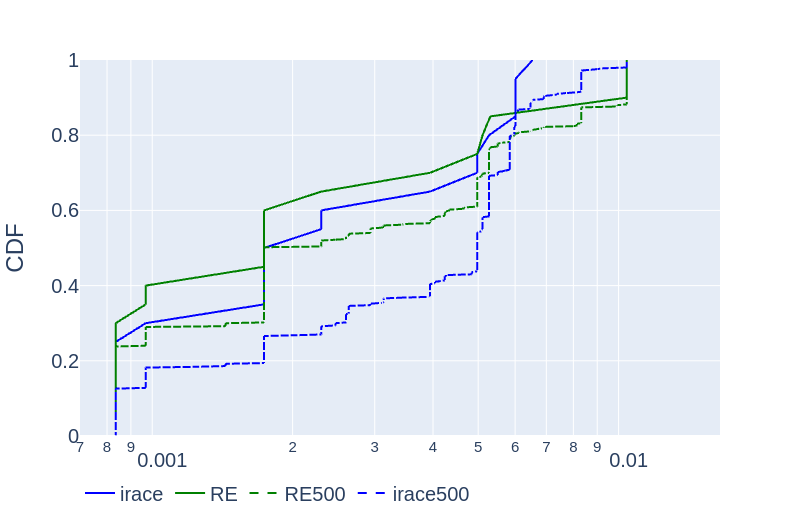
\includegraphics[width=0.8\linewidth, clip=true, trim=45px 20px 75px 50px]{imgs/ecdf-repetitions.png}
\caption{Empirical cumulative distribution function~($x$-axis) of the mean final regret~($y$-axis) assessing the effect of reducing the number of repetitions from 500~(dashed) to 20~(solid) for selected algorithms. Green: RE; blue: irace.}
\label{fig:ecdf-repetitions}
\end{figure}

\subsection{Comparing Algorithms for Final Quality}
%\leslie{}{[I think this should go in the next section, no?]} 
Figure~\ref{fig:ecdf-original} depicts the ECDFs for final quality, measured as mean test regret, of 20 runs of \irace, RE, and SMAC. Once again, all algorithms are run under the setup described in the \nasbench proposal with the exception of the number of runs, reduced for these experiments from 500 to 20.
Concerning SMAC, results differ w.r.t. the original \nasbench assessment given a change we adopt in the evaluation for comparison fairness. Specifically, the original assessment of SMAC considered a single evaluation of each configuration arguing that this led to faster convergence than multiple evaluations. We believe that this faster convergence is an effect of the limited variability provided by \nasbench and thus using such strategy may benefit all algorithms. As we will discuss in the following sections, that approach not only speeds convergence for SMAC, but leads to an improvement in its anytime performance. %Nevertheless, we remark that running SMAC with single evaluation for 20 runs produces an ECDF that follows a pattern similar to the ECDF reported in \nasbench for 500 runs.
\begin{figure}[!t]
\centering
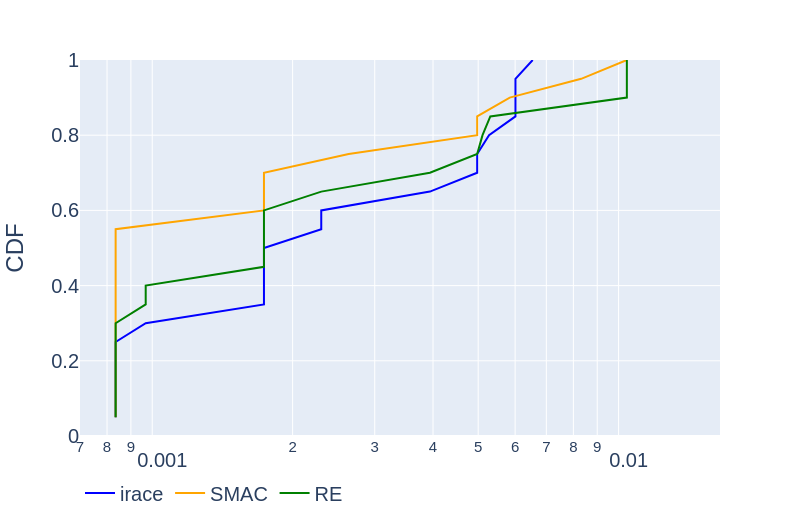
\includegraphics[width=0.8\linewidth, clip=true, trim=45px 20px 75px 50px]{imgs/ecdf-fnn-nocache.png}
\caption{Empirical cumulative distribution function~($x$-axis) of the final regret~($y$-axis) from 20 runs of each algorithm.}
\label{fig:ecdf-original}
\end{figure}

Concerning results given in Figure~\ref{fig:ecdf-original}, the comparison between \irace and the remaining algorithms shows that RE and SMAC are able to find better-performing architectures more often than \irace. However, \irace less often returns poor-performing architectures compared to RE and SMAC. Interestingly, SMAC outperforms not only \irace, but also RE, which had not been reported in the \nasbench evaluation. We believe this is due to the single versus multiple evaluation per candidate previously discussed, as follows. In~\cite{YinKleChrReaMurHut2019nasbench}, authors report that single evaluation speeds up convergence for SMAC. In search optimization, it is rather common that improving convergence speed without accounting for anytime performance leads to a decrease in final-quality performance. In addition, it is important to remark that the stopping criterion adopted does not include CPU time, hence the overhead incurred by learning in SMAC is not accounted for. 

For overall conclusions, we compare algorithms based on the area between their ECDF and the y-axis. The smaller the value, the better the performance of the algorithm.
%, indicating that every run from an algorithm achieved the minimum regret available in the benchmark. 
Table~\ref{tab:ecdf} groups results by experimental setup~(top) and algorithm~(bottom). The original setup discussed in this section is labeled~\textbf{O}~(\textit{original}). For this setup, SMAC is the best-ranked algorithm, followed by \irace and RE.
%In more detail, the AUC of the ECDF for each algorithm under each setup is given in parentheses. Results are groupby by experimental setup~(top) or algorithm~(bottom). 
We performed a Friedman non-parametric test with 98\% confidence and Nemenyi's posthoc test. When statistical significance is observed, best-ranked levels in Table~\ref{tab:ecdf} are highlighted in boldface, along with algorithms that are not statistically different to them.
Under the setup considered in this section, no statistical difference between the algorithms can be observed. 

\subsection{Evaluation Variability }
\label{sec:caching}
As previously discussed, the performance estimation required to assess the quality of an architecture requires multiple evaluations to be precise. 
%On the other hand, fewer evaluations are required when smaller variance is observed.} 
In \nasbench, the variability of the evaluations of the sampled architectures is represented only by three evaluation seeds. 
%\leslie{over only one data set}{}. \leslie{}{ 
Given this characteristic of \nasbench, we can consider storing evaluation results~(caching) to use the saved TPU time to evaluate more candidate architectures. 
This is essentially equivalent to the evaluation strategy defined in the experimental setup of SMAC in the original evaluation of \nasbench. In this section, we assess algorithms setting to one the maximum number of evaluations per architecture.
Though only SMAC has a hyperparameter to limit the number of function evaluations per configuration, we implement caching within the benchmark querying API for RE and \irace. 
%was set to one allowing only one evaluation as performance measure.

Table~\ref{tab:ecdf} shows results for the setup discussed in this section labeled as \textbf{C}~(short for \textit{caching}). 
Results grouped by experimental setup~(top) show that the relative performance of the algorithms is not altered by this factor alone. Yet, results grouped by algorithm~(bottom) demonstrate that the performance of all algorithms is much worsened when the caching strategy is adopted, though no statistical difference is observed w.r.t. other setups. We remark that \irace and RE were originally configured for the setup without caching, which could affect their performance in the caching setup. Interestingly, SMAC performs better by not using caching even having been configured for the caching setup in the original \nasbench assessment. Furthermore, it is also important to remark that \irace bases its search on statistical tests, which require variability to work. In a sense, though caching allows \irace to better explore the NAS search space, it also impairs the exploitation capability of the algorithm.
% RE, in particular, presents its worse performance among all experimental setups considered. Interestingly, if caching and variable-size encoding are adopted simultaneously, SMAC is able to achieve its best results among all experimental setups, and the performance of RE is not as poor as before. Conversely, \irace presents its worst performance. 
%Altogether, the results summarized in Table~\ref{tab:ecdf}~(bottom) evidence how different experimental design choices can have different effects on the final performance of these NAS algorithms. 

\begin{table}[!t]
    \centering
        \caption{ECDF analysis grouped by experimental setup~(top) and algorithm~(bottom). O: original; VS: variable-sized; C: caching; CVS: caching \& variable-sized. Best-ranked levels are highlighted when statistically different than the others. Values in parentheses are multiplied by $10^{4}$.}
    \label{tab:ecdf}

    \scalebox{0.825}{
    \begin{tabular}{r|r|r|r}
    \toprule
     O $\,$ & SMAC (23)$\,$ & $\,$\irace (28)$\,$  & RE (31)$\,$  \\
    \midrule
    VS $\,$ & $\,$\textbf{SMAC (18)}$\,$ & $\,$\irace (46)$\,$ & RE (47)$\,$ \\
    \midrule
    C $\,$ & $\,$ SMAC (34)$\,$ & $\,$\irace (50)$\,$ & RE (55)$\,$ \\
    \midrule
    CVS $\,$ & $\,$ \textbf{SMAC (20)}$\,$ & $\,$\irace (42)$\,$ & $\,$ RE (50)$\,$ \\
    \bottomrule
    \end{tabular}
    }
    \\[1em]
    \quad
    \scalebox{0.85}{
        \begin{tabular}{r|r|r|r|r}
        \toprule
            RE$\,$ & O (31) & VS (47) & $\,$CVS (50) & C (55)  \\
        \midrule
            \irace & O (28) & $\,$CVS (42) & VS (46) & C (50) \\
        \midrule
            SMAC$\,$ & $\,$ VS (18) & CVS (20) & O(23) & C (34)  \\
        \bottomrule
            % \multicolumn{5}{c}{}\\[0.17cm]
        \end{tabular}
}\end{table}

%%%
%%%
%%%
%%%
\subsection{Including the Number of Nodes in the Design Space}
The design space adopted in the original \nasbench considers a fixed-size encoding of
network architecture. It is important to note that, though the encoding is fixed-size, 
the final architecture they encode is variable in size. Yet, search algorithms are blind to this 
decoupling between architecture and its representation. We then include the number of
nodes as a parameter in the design space that determines the dimensions of
the adjacency matrix and node label list. Concerning final-quality ECDF analysis grouped by
experimental setup given in Table~\ref{tab:ecdf}~(top) for this setup~(labeled \textit{variable-sized}, \textbf{VS}), the relative performance of the algorithms is not affected. Yet, SMAC is now able to significantly outperform the remaining algorithms. In more detail, results grouped by algorithm~(bottom) show that SMAC greatly benefits from the variable-sized approach, whereas RE and \irace worsen their performance. 

Regarding RE and SMAC, these results are consistent with our previous discussion on the benefits of ACs. In more detail, the variable-size approach poses higher difficulty due to the larger parameter space and/or the conditional dependencies incurred by the new parameter. Under this setup, RE mutation might not be as adequate for the new design space and the algorithm is not able to define as good search trajectories as before. Conversely, ACs have been devised for scenarios that include this kind of parameter, and the performance of SMAC reflects this. Concerning \irace, we conjecture that the different probability modeling approaches adopted by SMAC (global) and \irace (local) account for the differences in performance between these algorithms for this setup. In addition, we remark that algorithms have been configured for the original setup, and hence an assessment of this encoding using reconfigured algorithms could likely alter our conclusions.

We conclude our preliminary final-quality assessment highlighting that the combination of caching and variable-sized encoding~(a setup labeled \textbf{CVS}) reveals interactions between these factors. In more detail, Table~\ref{tab:ecdf} shows that combining caching with variable-sized encoding improves over using each of these factors individually for \irace. Conversely, for RE and SMAC, caching reduces the benefits of the variable-sized encoding, even if to a much smaller extent than when we compare the original setup with using caching alone.

% \leslie{\medskip In the next section, we assess how an anytime performance perspective affects the results discussed in this final-quality preliminary assessment.}{}
% %%%
%%%
\section{Assessing Anytime Performance}
\label{sec:anytime}
%\subsection{Benchmarking \irace and anytime assessment}

% and no statistically significantly differences can be found w.r.t. RE and \irace, using Friedman's non-parametric test with a confidence level of 98\%. %RE~(0.0022) and \irace~(0.0024) find high-performing architectures with similar probability, the performance of SMAC falls short~(0.0056). 
%Under this setup, \irace ranks last in the comparison to the remaining algorithms.
%Though \irace ranks last, our later discussion on alternative experimental setups willconfirm that \irace is a viable approach to \nasbench. 

As discussed in Section~\ref{sec:guidelines}, an assessment based solely on final quality excludes from the analysis the time required to achieve a given performance level. In this section, we perform an anytime comparison of all algorithms to investigate how their search dynamics differ. We also discuss the anytime effects of caching and of the variable-sized encoding. 


%, we compare the results based on the hypervolume indicator.
\subsection{Comparing Algorithms for Anytime Performance}
\begin{figure}[!t]
\centering
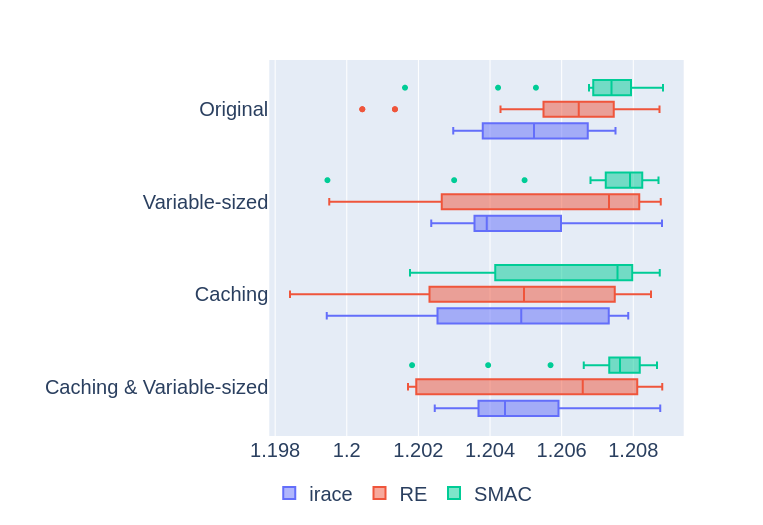
\includegraphics[width=0.9\linewidth, clip=true, trim=40px 20px 0 50px]{imgs/boxplots.png}
\caption{Boxplots of the hypervolume~($x$-axis) obtained in 20 runs from each of the algorithms selected, depicted in varying colors. Boxplots are grouped along the $y$-axis by the experimental setup adopted.}
\label{fig:boxplots}
\end{figure}

Figure~\ref{fig:boxplots} gives  boxplots of the hypervolume achieved by the algorithms in which runs are grouped by the experimental setup adopted. The smaller the value achieved, the better the anytime performance of the algorithm. The hypervolume indicator requires a reference point, and as traditionally done in the literature we use point $(2.1, 2.1)$. To do so, we initially normalize results to the $[1,2]$ range respectively using $[0,10^7]$ and $[0,1]$ as bounds for TPU time and mean test regret. 

For the original setup adopted in \nasbench, we observe intersections between the boxplots, though clearly SMAC outperforms \irace. This is confirmed by the rank sums given in Table~\ref{tab:rs-anytime}~(top), where SMAC is followed by RE and \irace ranks last. Interestingly, the variance in results increases in this order as well. The relative rankings observed for anytime performance contrast with the rankings observed for final quality in Table~\ref{tab:ecdf}~(top), where \irace ranked better than RE. The poor anytime performance of \irace is related to the budget set for each iteration, which is directly affected by the hyperparameters we configured for final-quality assessment. 
% no statistical significant difference can be found among all algorithms 
% %and no statistically significantly differences can be found w.r.t. RE and \irace, 
% using Friedman's non-parametric test with a confidence level of 98\%. 

\begin{table}[!t]
    \centering
    \caption{Rank sum (RS) analysis of hypervolumes grouped by experimental setup~(top) and algorithm~(bottom). O: original; VS: variable-sized; C: caching; CVS: caching \& variable-sized. Best-ranked levels are highlighted when statistically different different than others.}
    \label{tab:rs-anytime}
    \scalebox{0.85}{
    \begin{tabular}{r|r|r|r}
    \toprule
     O $\,$ & \bf{SMAC (30)}$\,$ & $\,$ \bf{RE (37)}$\,$  & $\,$ \irace (53) \\
    \midrule
    VS $\,$ & $\,$ \bf{SMAC (30)} & \bf{RE (40)}$\,$ & $\,$ \irace (50)  \\
    \midrule
    C $\,$ & $\,$ SMAC (32)$\,$ & RE (43)$\,$ & $\,$ \irace (45) \\
    \midrule
    CVS $\,$ & \bf{SMAC (30)}$\,$ & $\,$\bf{RE (43)}$\,$ & $\,$ \irace (47) \\
    \bottomrule
    \end{tabular}
    }\\[1em]
    \quad
    \scalebox{0.85}{
        \begin{tabular}{r|r|r|r|r}
        \toprule
            RE$\,$  & VS (47) & O (48) & CVS (49) & C (56)  \\
        \midrule
            \irace & O (45) & CVS (48) & C (52) & CVS (55) \\
        \midrule
            SMAC$\,$ & VS (43) & CVS (46) & O (54) & C (57)  \\
        \bottomrule
            \multicolumn{5}{c}{}\\[0.17cm]
        \end{tabular}
}\end{table}

We then compare the two best-performing algorithms, i.e., RE~(left) and SMAC~(right), with the help of empirical attainment function~(EAF) difference plots, given in Figure~\ref{fig:eaf-original}. As previously discussed, the $x$-axis depicts TPU time only, whereas the $y$-axis gives mean test regret. Dashed lines depict the 50\% attainment function from each algorithm, and differences depicted as shaded areas on either side of the plot indicate that the given algorithm presented a better performance at that point of the runs. 
RE is designed for this type of configuration scenario, favoring a quick intensification of the search. On the other hand, SMAC requires more TPU time to obtain a similar level of performance. This is the consequence of the evaluation strategy implemented by SMAC which, despite the low variability inherent to \nasbench, assumes the estimation of architecture performance to require several executions to be accurate. Hence, RE has a higher probability of obtaining best performance than SMAC with a lower TPU time budget, while for higher TPU times SMAC provides a better probability. If CPU-time were accounted for, however, the conclusions drawn from this comparison would likely be affected by the sequential nature of SMAC.
%These results highlight the benefits and pitfalls of the different search strategies implemented by SMAC and RE, providing a more accurate picture of their overall performance.

\begin{figure}[!t]
\centering
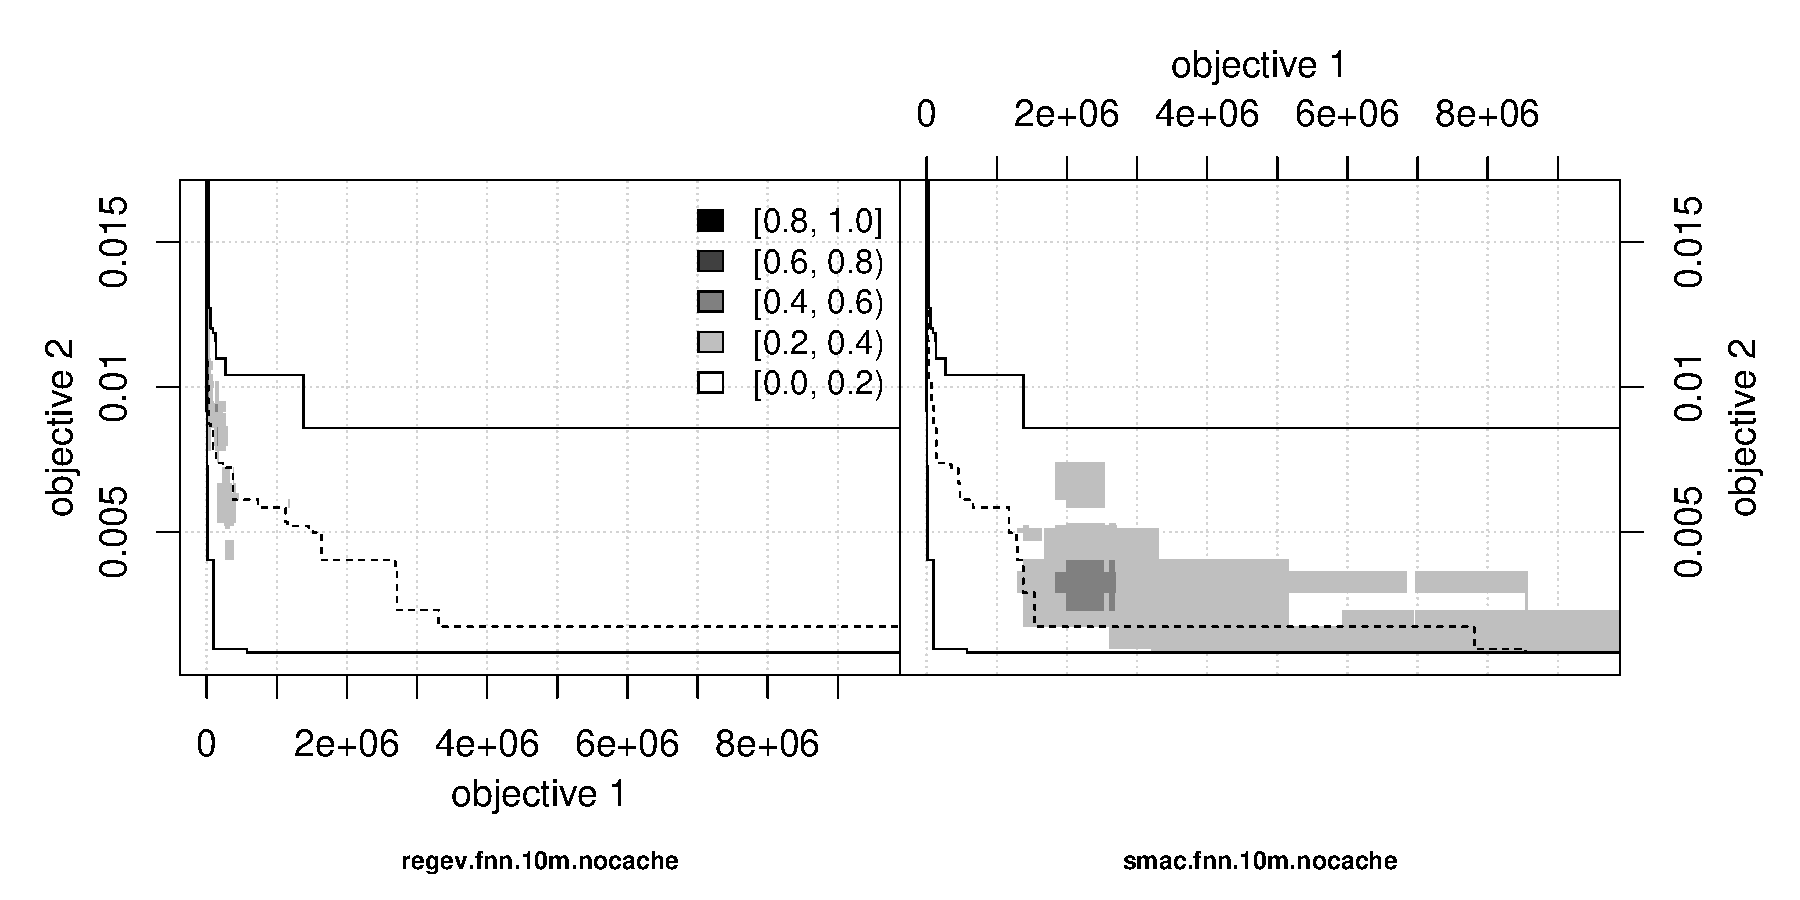
\includegraphics[width=\linewidth, clip=true, trim=45px 65px 85px 85px]{imgs/eaf-regev-smac-fnn-nocache.pdf}
\caption{Empirical attainment function~(EAF) difference plots comparing RE (left) and SMAC (right) run 20 times each. $x$-axis: TPU time; $y$-axis: mean test regret. %Dashed lines depict the 50\% attainment function from each algorithm. Differences depicted as shaded areas on either side of the plot indicate that the given algorithm presented a better performance at that point of the runs.
}
\label{fig:eaf-original}
\end{figure}

\subsection{Caching and Variable-Sized Encoding Effects}
The final-quality assessment discussed in the previous section showed that algorithm, variability degree, and solution encoding were interacting factors. Specifically, the only pattern observable in Table~\ref{tab:ecdf}~(bottom) referred to the caching strategy, which led to poor results for all algorithms when used with the fixed-size solution encoding. By contrast, Figure~\ref{fig:boxplots} shows that these alternative approaches affect most anytime performance as to the variance in the results. RE is the algorithm most affected, whereas SMAC is the least. Distribution shifts are also observed for all algorithms, though they vary as a function of the remaining factors. For SMAC and RE, the variable-sized encoding right-shifts the distributions, though a bit less in the presence of caching. Conversely, \irace presents its best anytime performance in the original \nasbench setup. 

The rank sum analysis given in Table~\ref{tab:rs-anytime} confirms these findings. On the top grouping, experimental setups do not alter the relative performance of the algorithms, though caching affects statistical significance due to the high variance in SMAC results discussed above. For the bottom grouping, rank sums for the different setups are very similar within each row, again due to the increased variance in results. As previously discussed, these conclusions should consider that all algorithms have been configured for final-quality optimization under the original setup. Yet, they further evidence the need for benchmarking NAS from an anytime performance perspective.

% A different pattern in boxplots is observed when we assess anytime performance for the variable-sized approach. For this setup, the variance in results is greatly increased for RE, whereas the distribution in SMAC is right-shifted. By contrast, the distribution of \irace presents a smaller As previously discussed for final-quality assessment, these results are consistent with our previous discussion on the benefits of ACs. \irace is unable to benefit here from this alternative setup. %Why??? I mean, who cares? :P
% Furthermore, though the increment in variance is much lower for \irace than for RE, the rank sum analysis given in Table~\ref{tab:ecdf}~(top) for this setup~(labeled VS) shows that RE is the least affected algorithm. This is likely explained by the changes in performances from the remaining algorithms and seed pairing, which the boxplots conceal. Yet, no statistically significant differences can be found among the algorithms once again.

% %The indicator is able to show clearly the differences performance between the algorithms. 
% % The hypervolume obtained by RE and \irace is significantly better than the obtained by SMAC (Wilcoxon test $\alpha=0.05$). While RE and \irace are close and the difference in their results is not significant.... \leslie{}{just inventing here...}

% Concerning anytime performance of caching evaluations, Figure~\ref{fig:boxplots} shows that caching indeed improves the performance of SMAC, as reported in the original \nasbench proposal. Yet, the remaining algorithms are negatively affected in variance and/or distribution shift. In the case of RE, we understand that an algorithm with strong convergence pressure benefits from variability to avoid early stagnation, and hence having longer to search does not help. As for \irace, having \leslie{}{the equivalent to} a single instance to work with greatly limits the benefits of seeing more configurations, as the statistical test used to discard races does not have enough evidence to work with. Though SMAC was also devised for multi-instance algorithm configuration, it is an extended version of an originally per-instance configurator, and hence it is better equipped to approach \nasbench. Nevertheless, the rank sum analysis provided in Table~\ref{tab:rs-anytime}~(top) for this setup~(labeled C) shows that all algorithms are considered statistically equivalent.

% If both caching and variable-sized encoding are considered at the same time, anytime results are a combination of the results seen for these individual factors. In more detail, SMAC improved its anytime performance when either caching or variable-sized encoding were adopted, so combined they lead SMAC to a significantly better performance than the remaining algorithms. \irace, especially, shows a performance deterioration even greater than RE. This is shown both in Figure~\ref{fig:boxplots} and Table~\ref{tab:rs-anytime}~(top), in which this setup is labeled CVS. The interactions between experimental design choices and algorithms are summarized in Table~\ref{tab:rs-anytime}~(bottom), where we see that RE is the algorithm least affected.
% \section{High-Performing Configuration Insights}
\label{sec:configurations}

\begin{figure*}[!t]
\centering
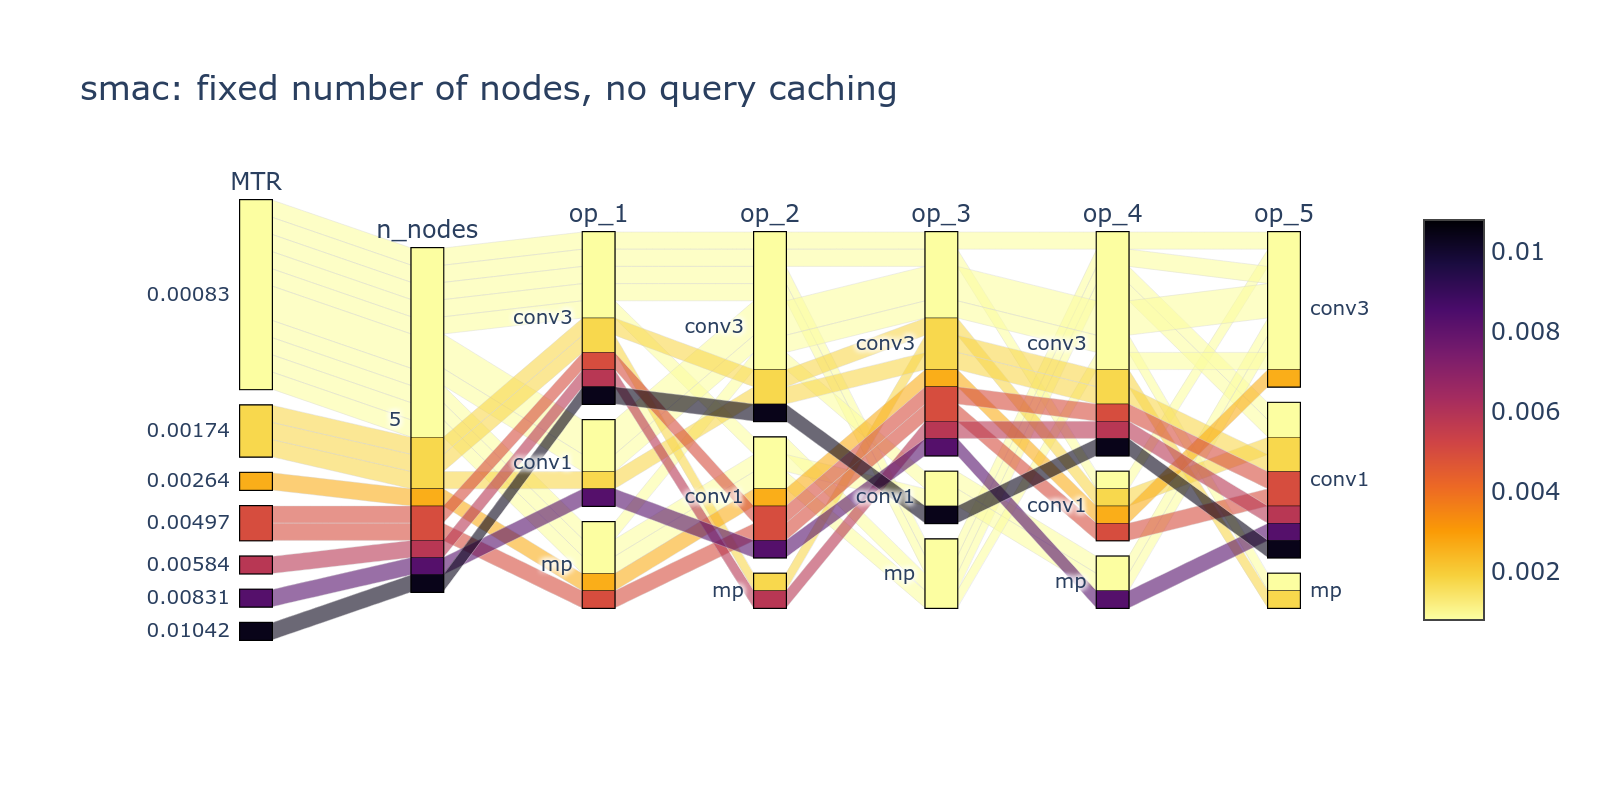
\includegraphics[width=0.47\linewidth, clip=true, trim=142px 155px 210px 170px]{imgs/parcat/smac-fnn-nc.png}
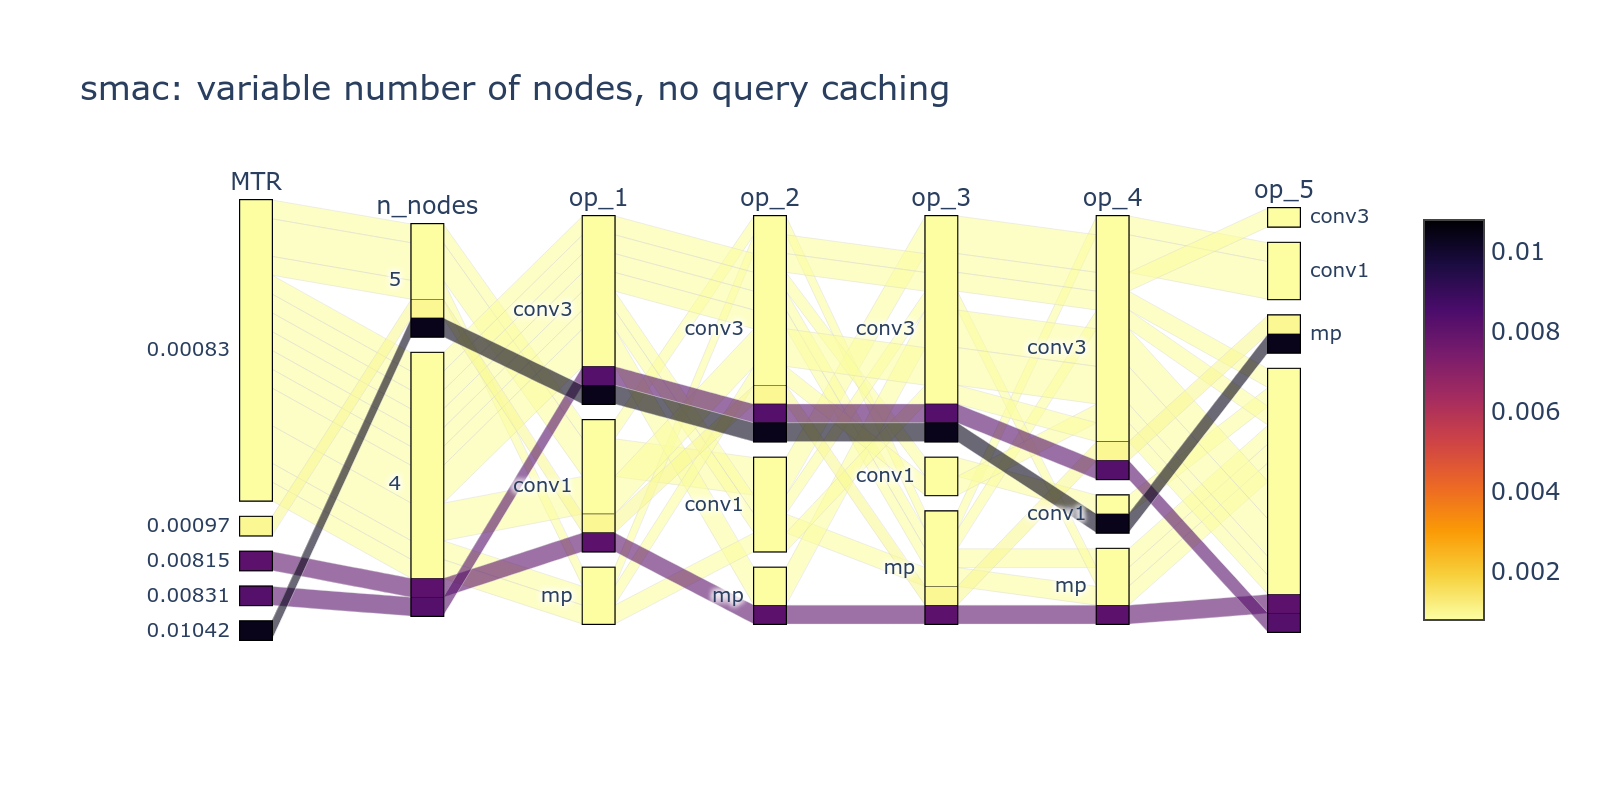
\includegraphics[width=0.51\linewidth, clip=true, trim=142px 155px 40px 170px]{imgs/parcat/smac-vnn-nc.png}
\caption{Parallel categories plots of the 20 architectures selected by SMAC with fixed (left) and variable (right) number of nodes.}
\label{fig:pc-smac}
\end{figure*}

In this section, we analyze the final configurations and thus, the architectures selected by the different NAS techniques. For this purpose, we study the configurations obtained in each run of the algorithms. Figure~\ref{fig:pc-smac} shows parallel categories plots for SMAC. For clarity, only NAS hyperpameters related to the node label list are given~(\textit{op$_1$}-\textit{op$_5$}).
% corresponding to each vertex of the DAG model, i.e. each layer of the selected neural network, for legibility's sake. 
The possible values for these parameters are \textit{conv3} ($3 \times 3$ convolution), \textit{conv1} ($1 \times 1$ convolution), \textit{mp} ($3 \times 3$ max-pooling), or empty in the case of the variable-sized approach. 
Since topology is defined by the adjacency matrix, no layer order or architecture size should be assumed.
Color scaling reflects the mean test regret, which we additionally depict as a discretized variable in the left-most column of the plot. Though conclusions in this section are drawn from all plots analyzed, the remaining ones 
%they are not all included here for brevity
% due to size restrictions, 
are given as supplementary material for brevity.

In line with the layer type performance effects reported in \nasbench, \textit{conv3} is the most frequently selected node value. This was especially true for \irace, particularly in the fixed-size approach. In fact, several of the high-performing configurations 
% across the board 
seem to use only \textit{conv3} nodes, with no \textit{conv1} nor pooling layers. This is surprising, as manual design would certainly include them. We believe that these results reflect the design for accuracy adopted in \nasbench. In particular, one of the most significant benefits from pooling is reducing training time. Yet, architectures are generally evaluated only as to their accuracy. Though it would be possible to assess some level of trade-off between architecture accuracy and total training time, we have followed the original setup from \nasbench where this is not considered. We remark, though, that this can lead to the selection of extremely costly architectures, such as the \textit{conv3}-based mentioned previously.
%which use only $3 \times 3$ convolutions.

Regarding caching, all algorithms have a hard time finding good configurations using this approach. This is a further indication of the usefulness of variability in this benchmark from a final-quality perspective. On the other hand, adopting a variable number of nodes can be beneficial, as is the case for SMAC. Yet, we remark that the architectures given in Fig.~\ref{fig:pc-smac} may present less than $n_\text{nodes}$ nodes due to their topology, which is not shown here. 
%Yet, we remark that the architectures given in Fig.~\ref{fig:pc-smac}~(left) may present less than five nodes due to their topology, which is not shown here. 
%This is also true for Fig.~\ref{fig:pc-smac}~(right), even if some architectures differ as to the NAS hyperparameter $n_\text{nodes}$. 
% the right-most a sepathat the variable approach allows SMAC to more easily find optimal configurations, which often have fewer than 5 nodes. This is not exclusive to SMAC, with other algorithms having their best configurations in the variable approach with 4 or 3 nodes,
Finally, we note that RE finds a top-performing configuration containing a single $1 \times 1$ convolution layer. We remark that this is possible due to the scalable architecture approach discussed in Section~\ref{sec:background}.

% \begin{figure*}[!t]
% \centering
% 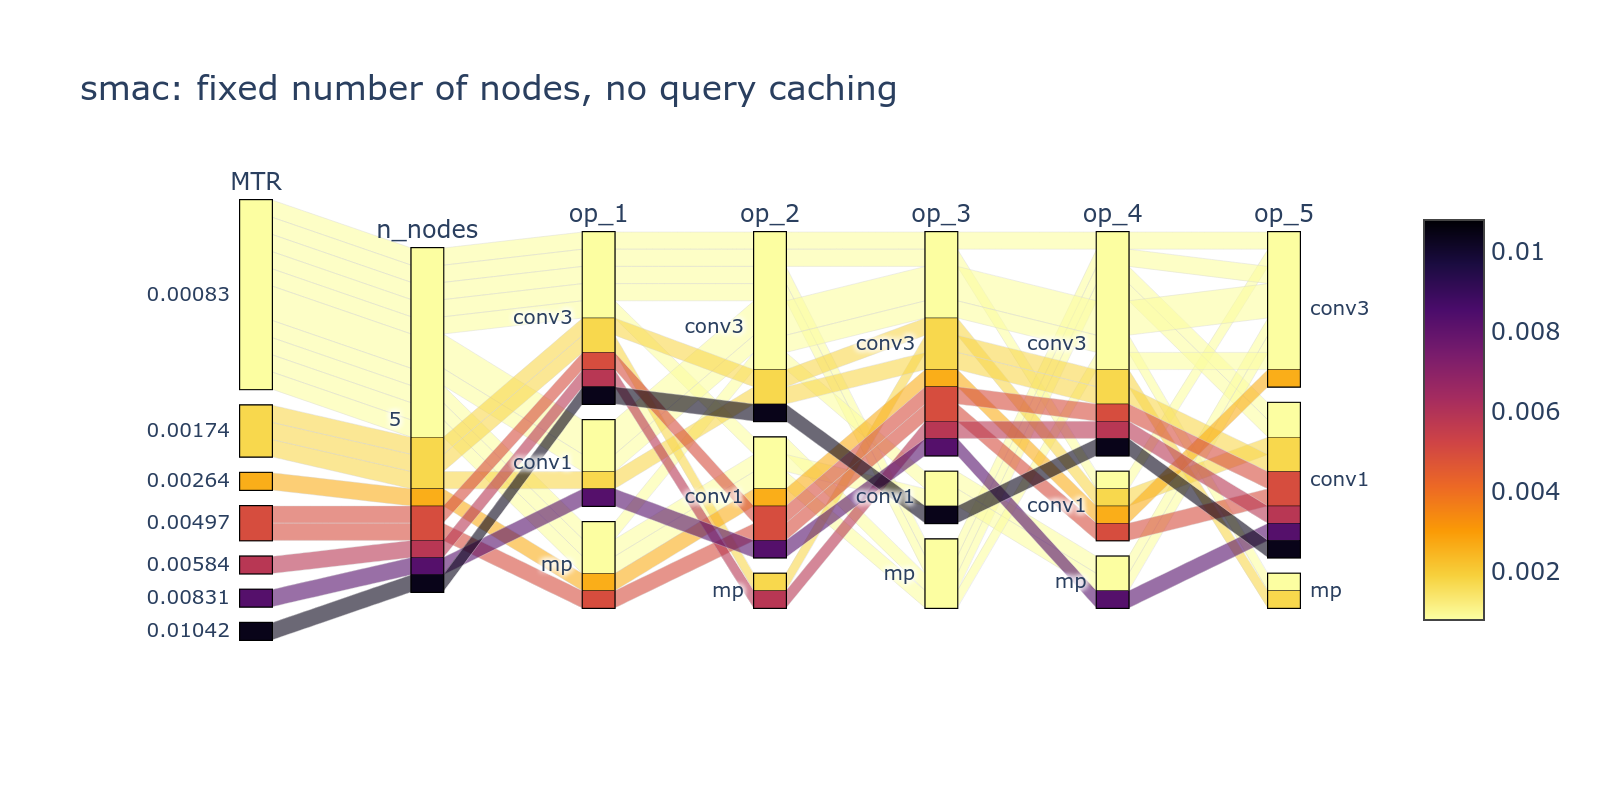
\includegraphics[width=0.47\linewidth, clip=true, trim=140px 150px 40px 150px]{imgs/parcat/smac-fnn-nc.png}
% 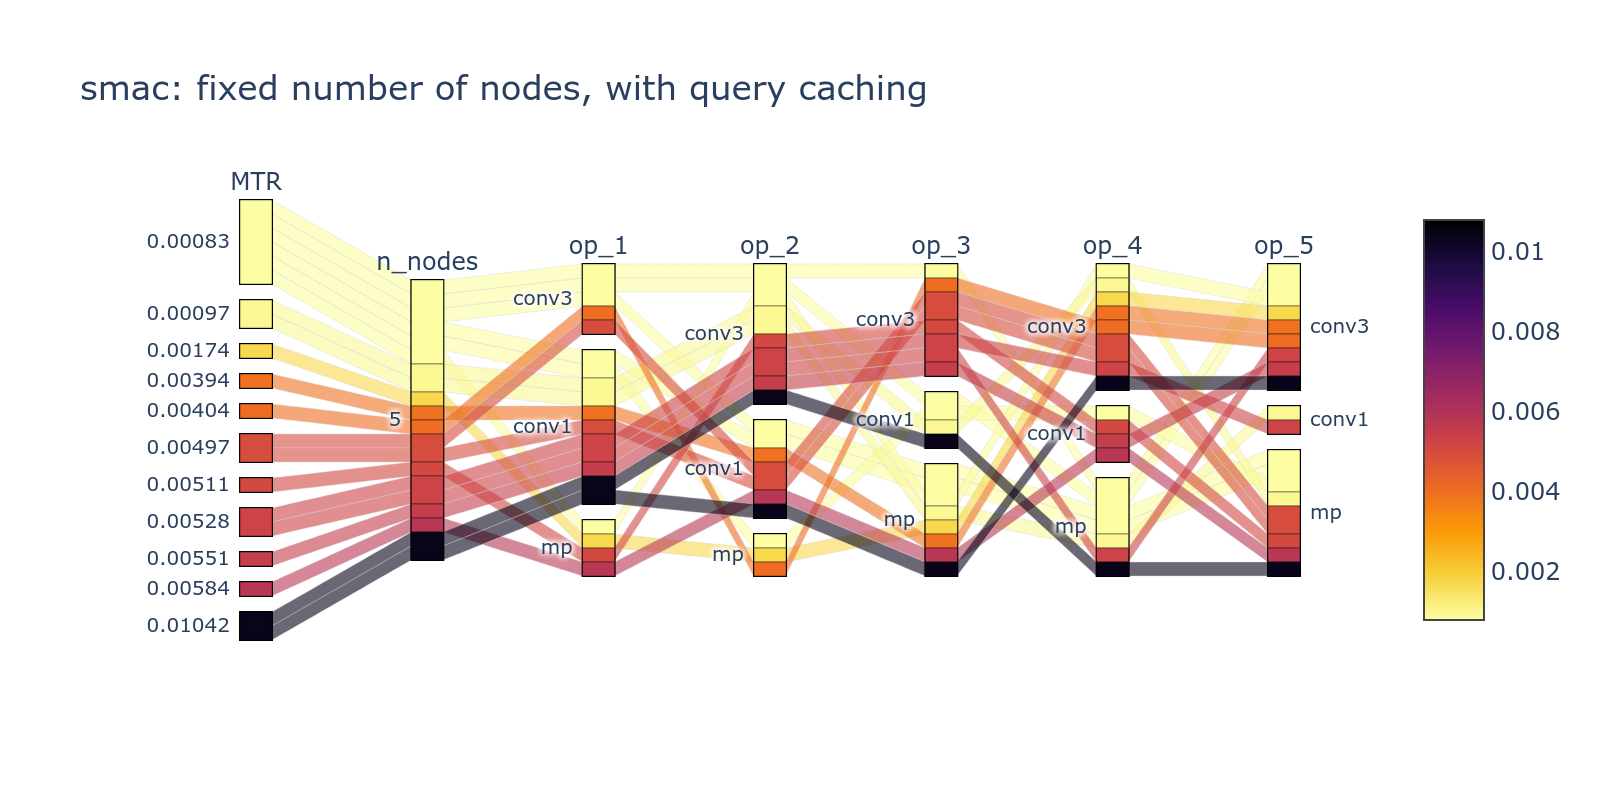
\includegraphics[width=0.47\linewidth, clip=true, trim=140px 150px 40px 150px]{imgs/parcat/smac-fnn.png}
% 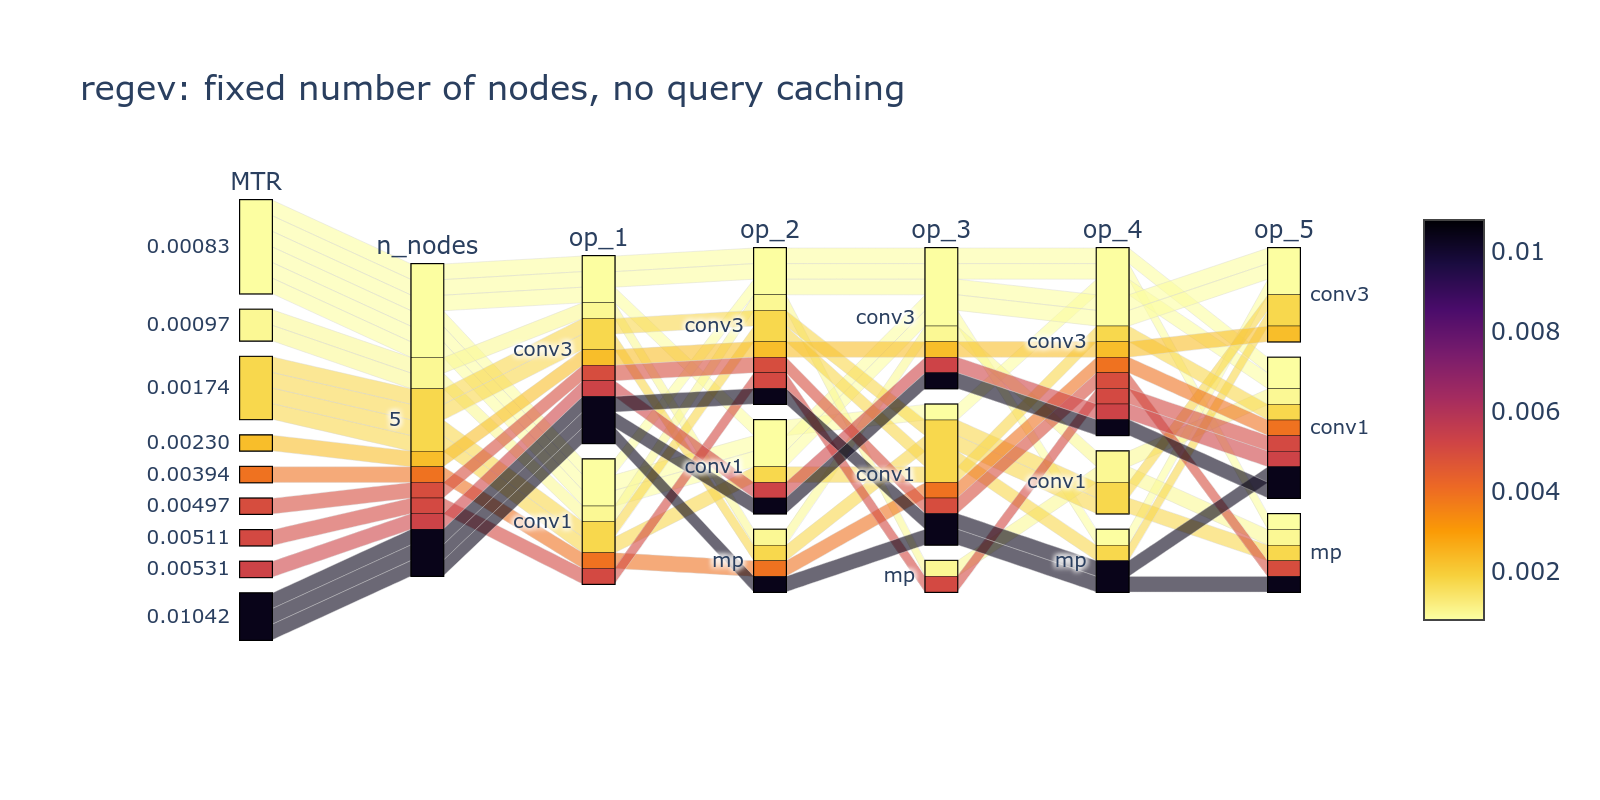
\includegraphics[width=0.47\linewidth, clip=true, trim=140px 150px 40px 150px]{imgs/parcat/re-fnn-nc.png}
% 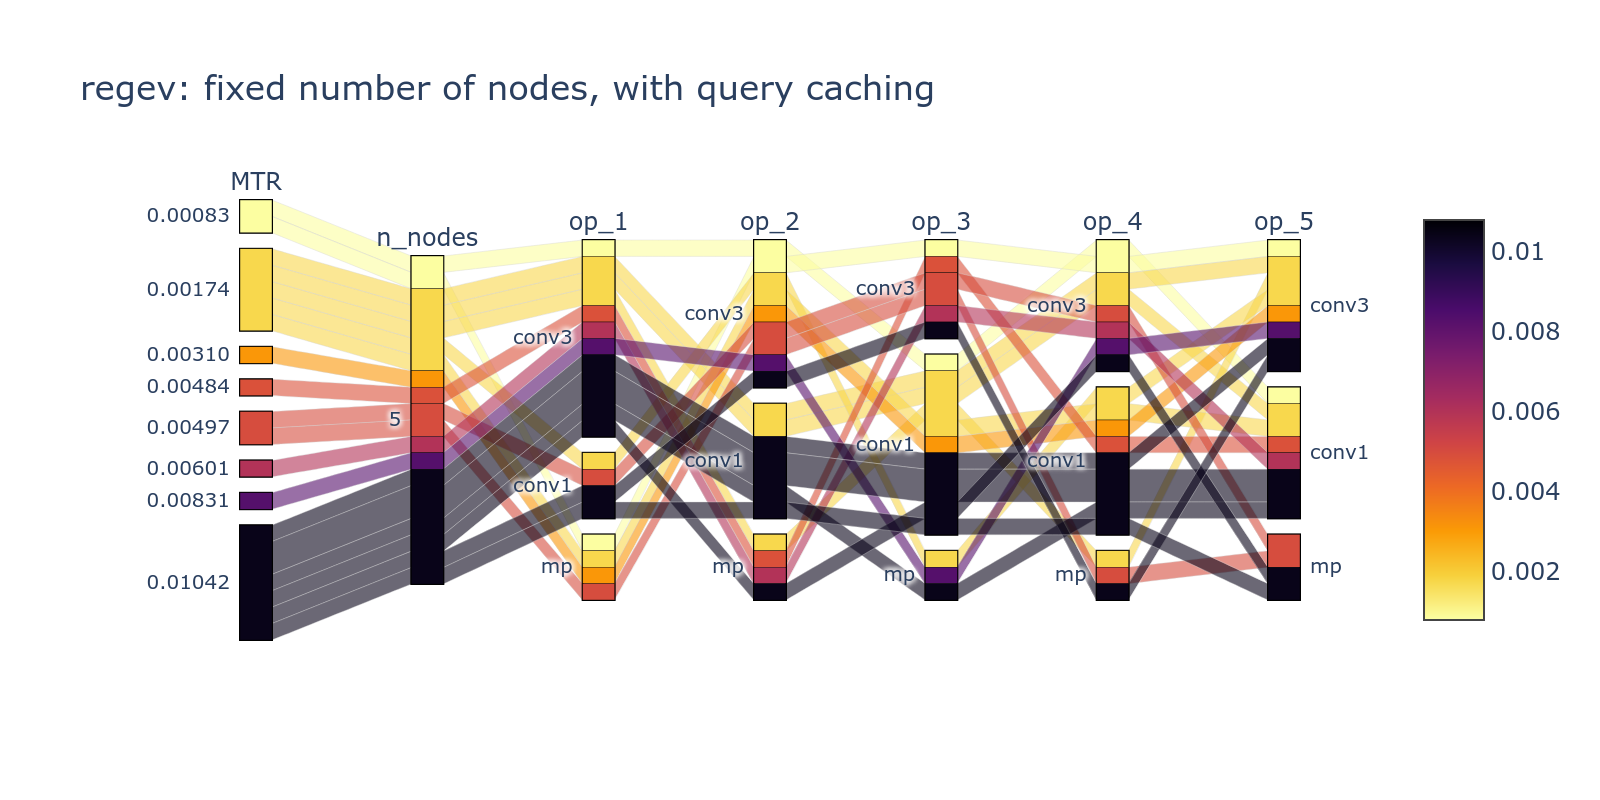
\includegraphics[width=0.47\linewidth, clip=true, trim=140px 150px 40px 150px]{imgs/parcat/re-fnn.png}
% 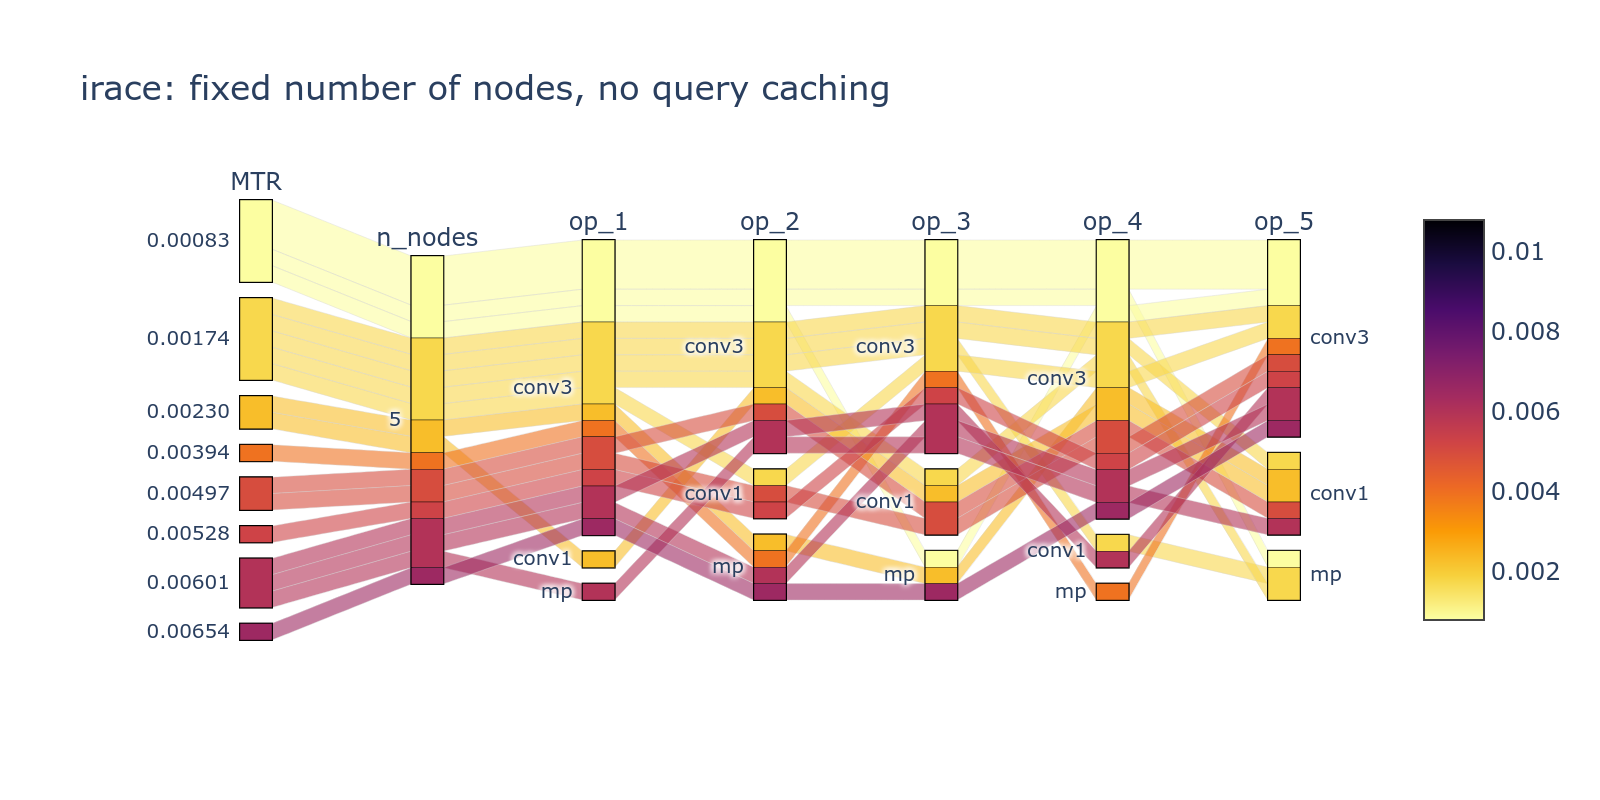
\includegraphics[width=0.47\linewidth, clip=true, trim=140px 150px 40px 150px]{imgs/parcat/irace-fnn-nc.png}
% 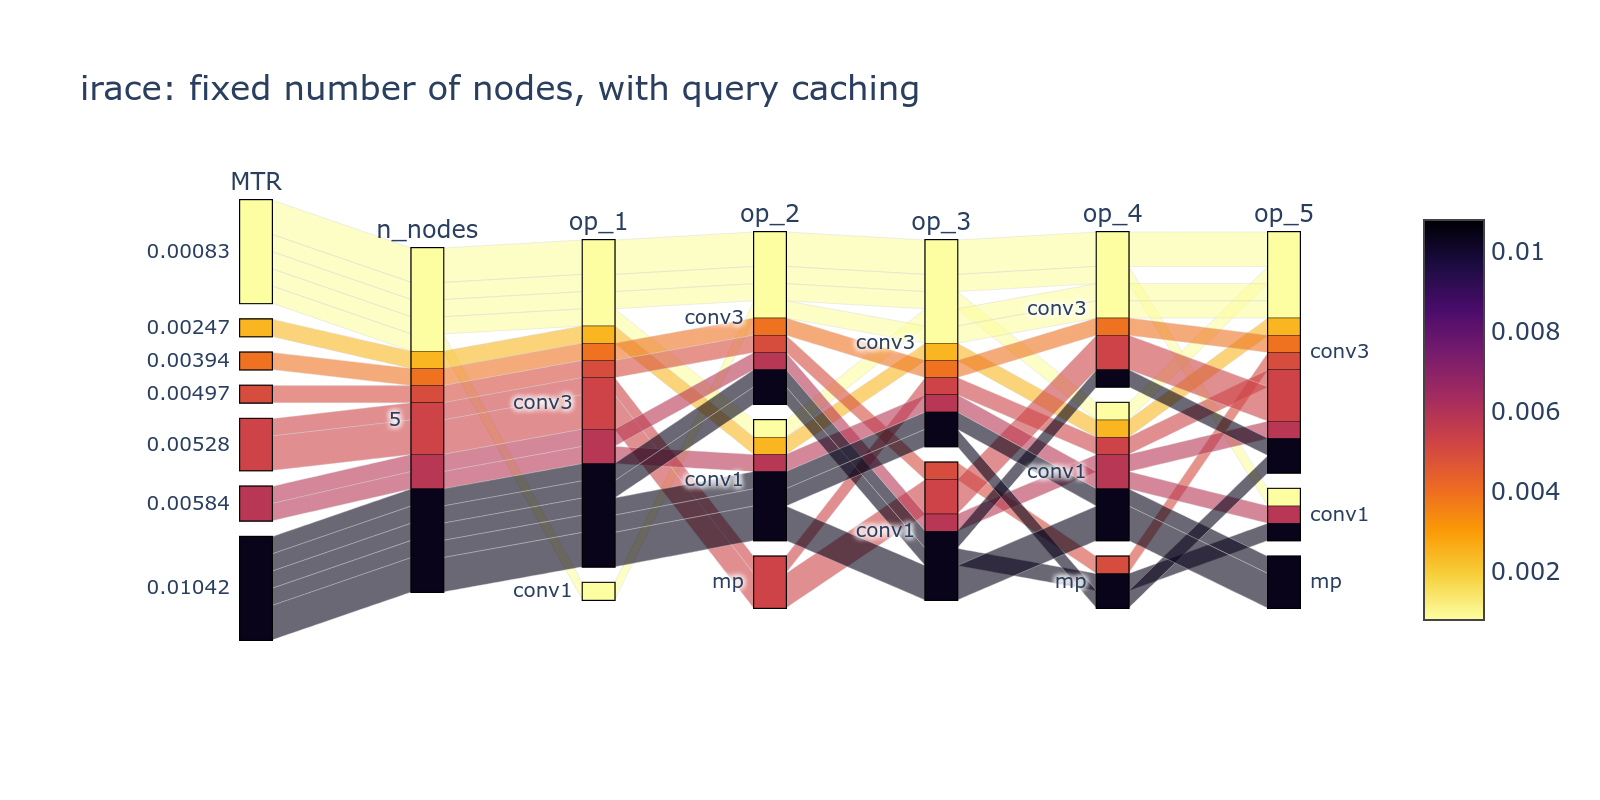
\includegraphics[width=0.47\linewidth, clip=true, trim=140px 150px 40px 150px]{imgs/parcat/irace-fnn.png}
% \caption{Parallel categories plots of the 20 architectures selected by SMAC (top), RE (middle), and \irace (bottom) with fixed number of nodes, no caching (left), caching (right).}
% \label{fig:cf-comp}
% \end{figure*}


% \begin{figure*}[!h]
% \centering
% 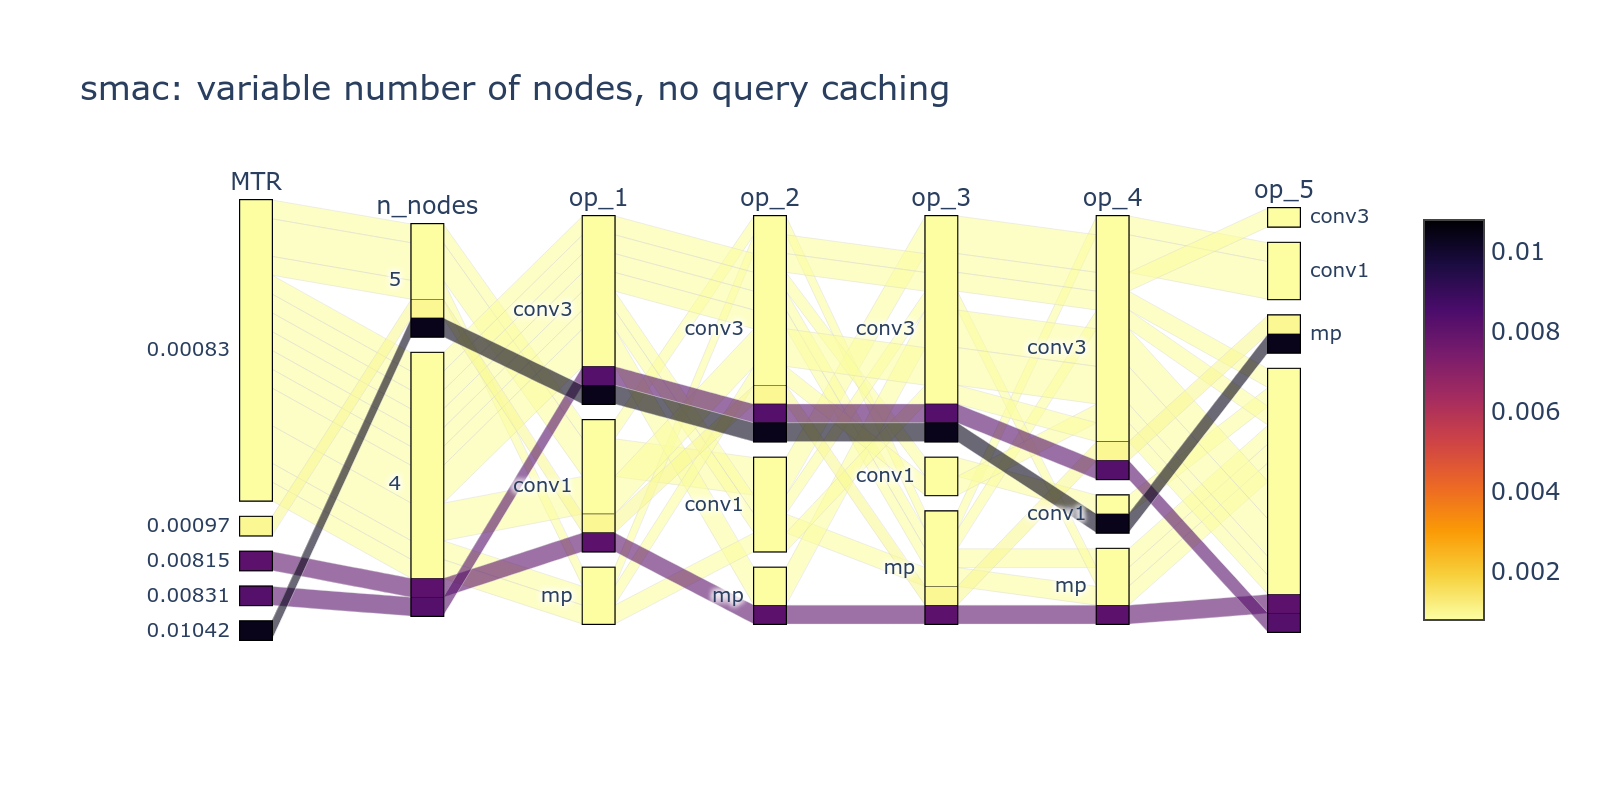
\includegraphics[width=0.47\linewidth, clip=true, trim=140px 150px 40px 150px]{imgs/parcat/smac-vnn-nc.png}
% 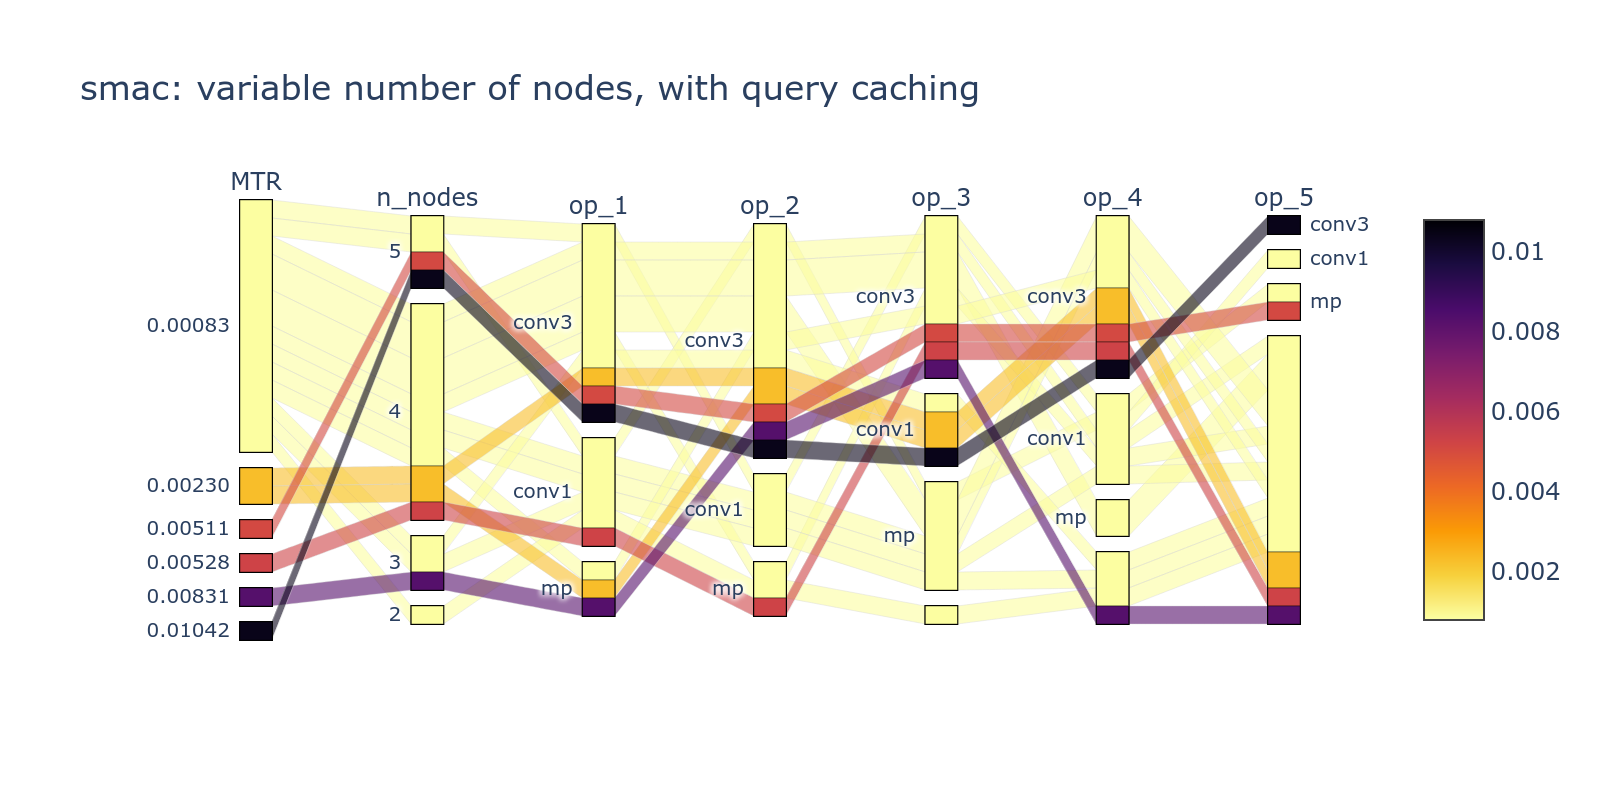
\includegraphics[width=0.47\linewidth, clip=true, trim=140px 150px 40px 150px]{imgs/parcat/smac-vnn.png}
% 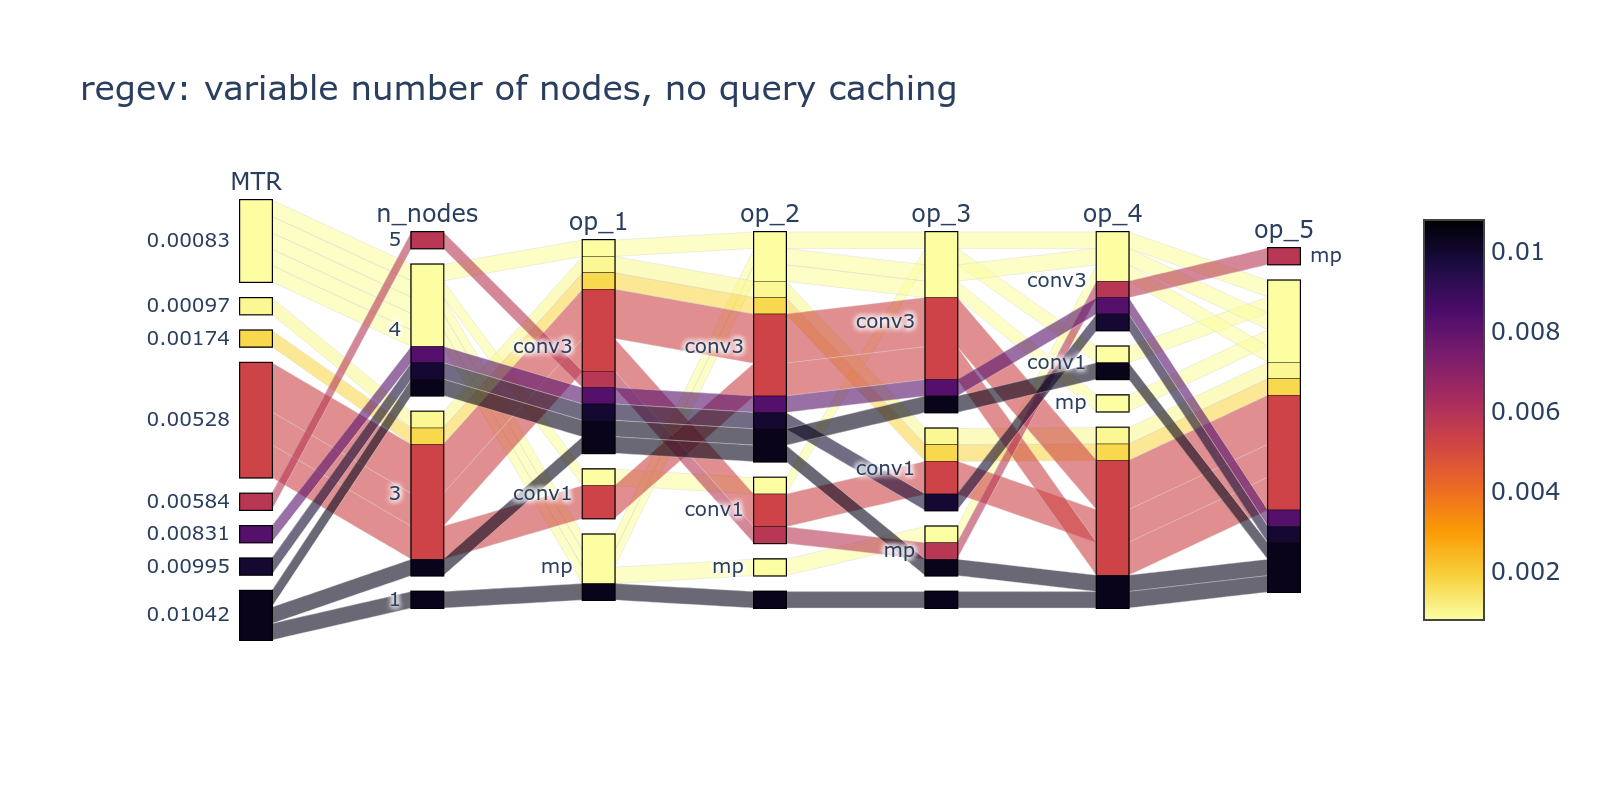
\includegraphics[width=0.47\linewidth, clip=true, trim=140px 150px 40px 150px]{imgs/parcat/re-vnn-nc.png}
% 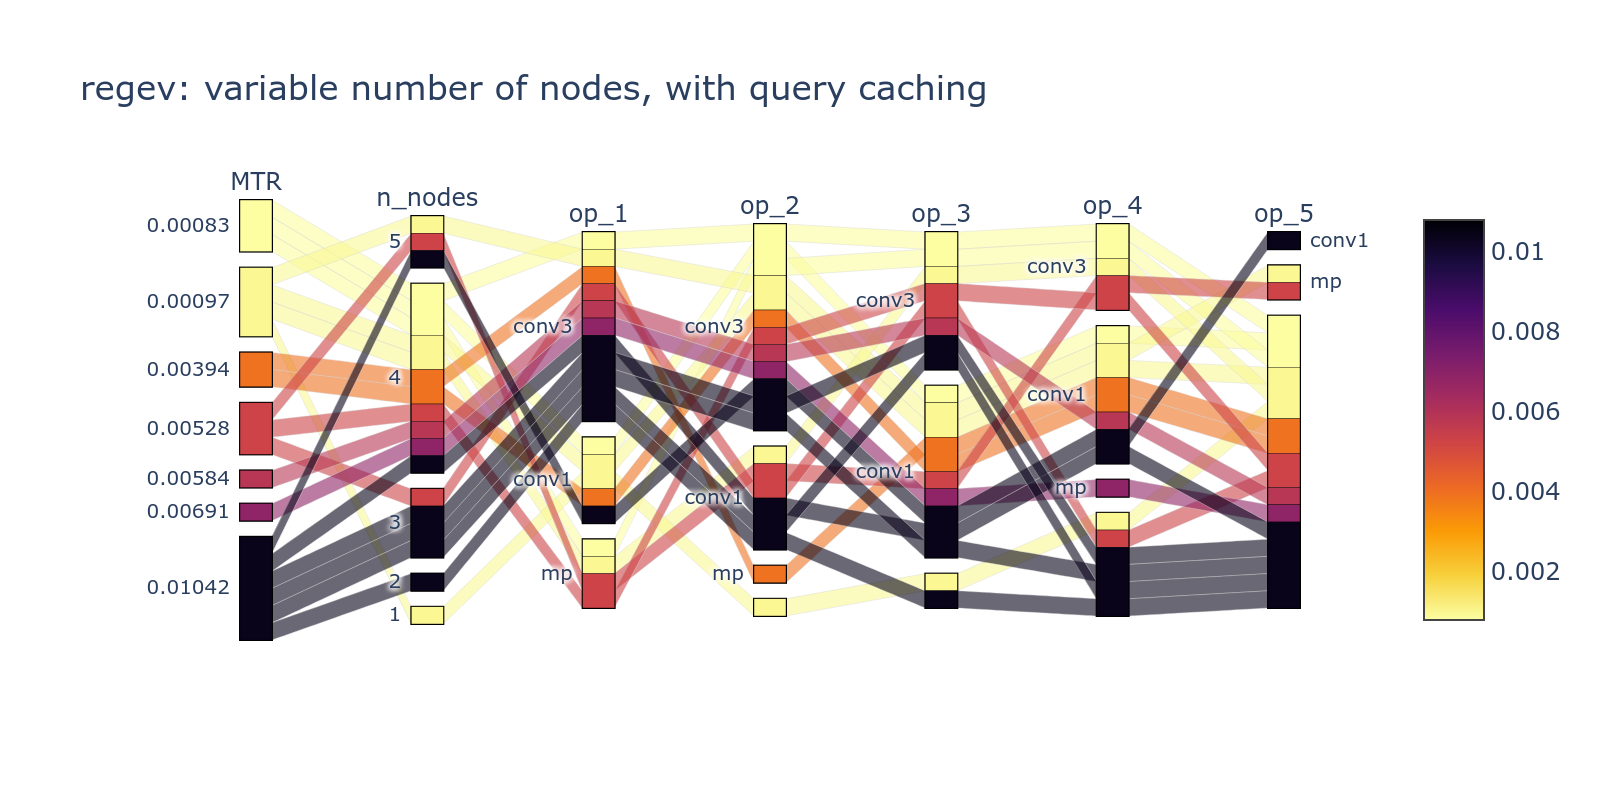
\includegraphics[width=0.47\linewidth, clip=true, trim=140px 150px 40px 150px]{imgs/parcat/re-vnn.png}
% 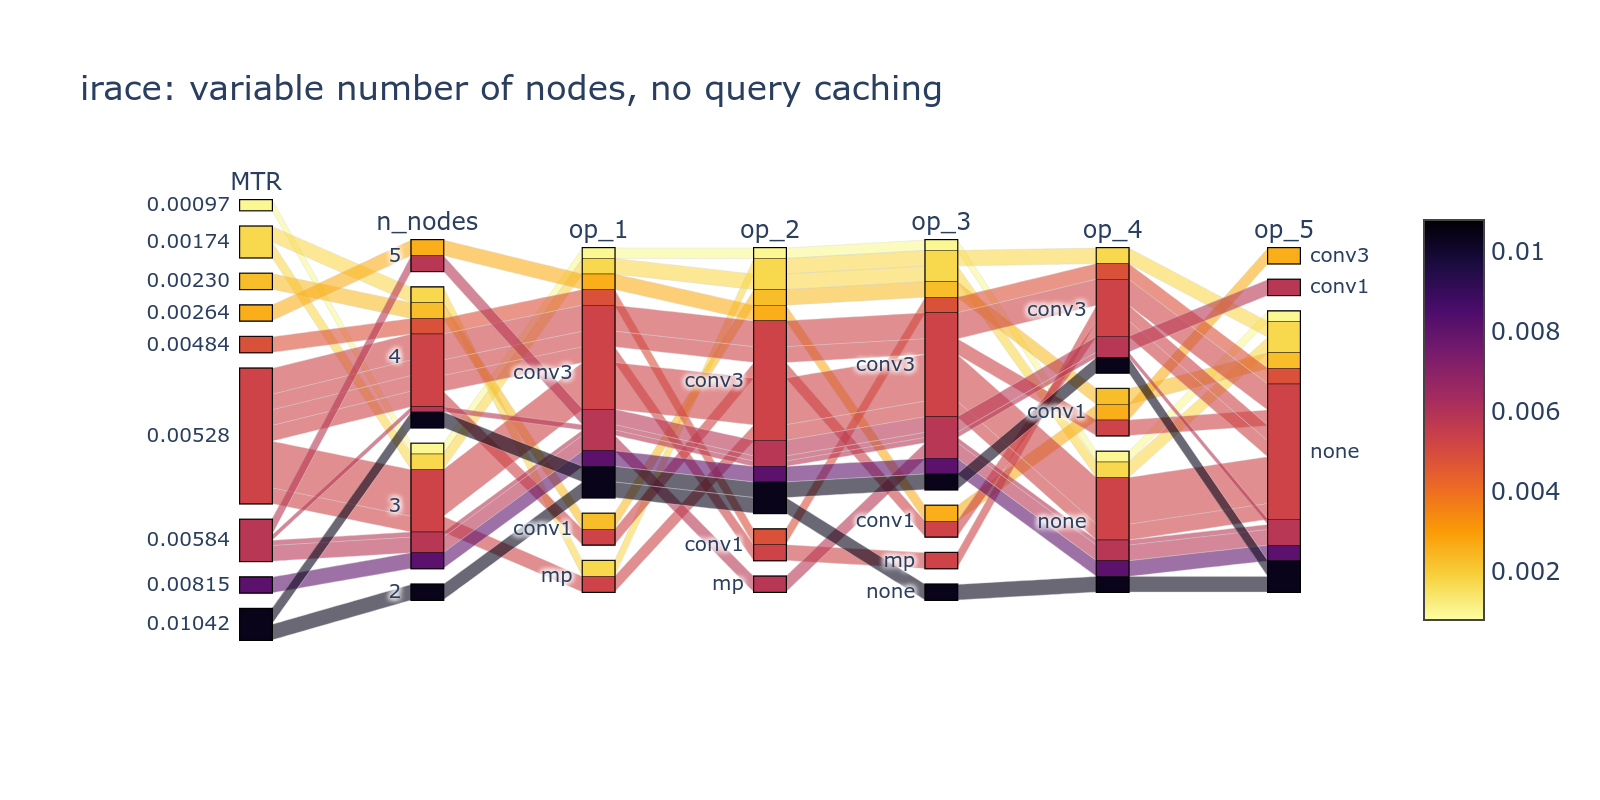
\includegraphics[width=0.47\linewidth, clip=true, trim=140px 150px 40px 150px]{imgs/parcat/irace-vnn-nc.png}
% 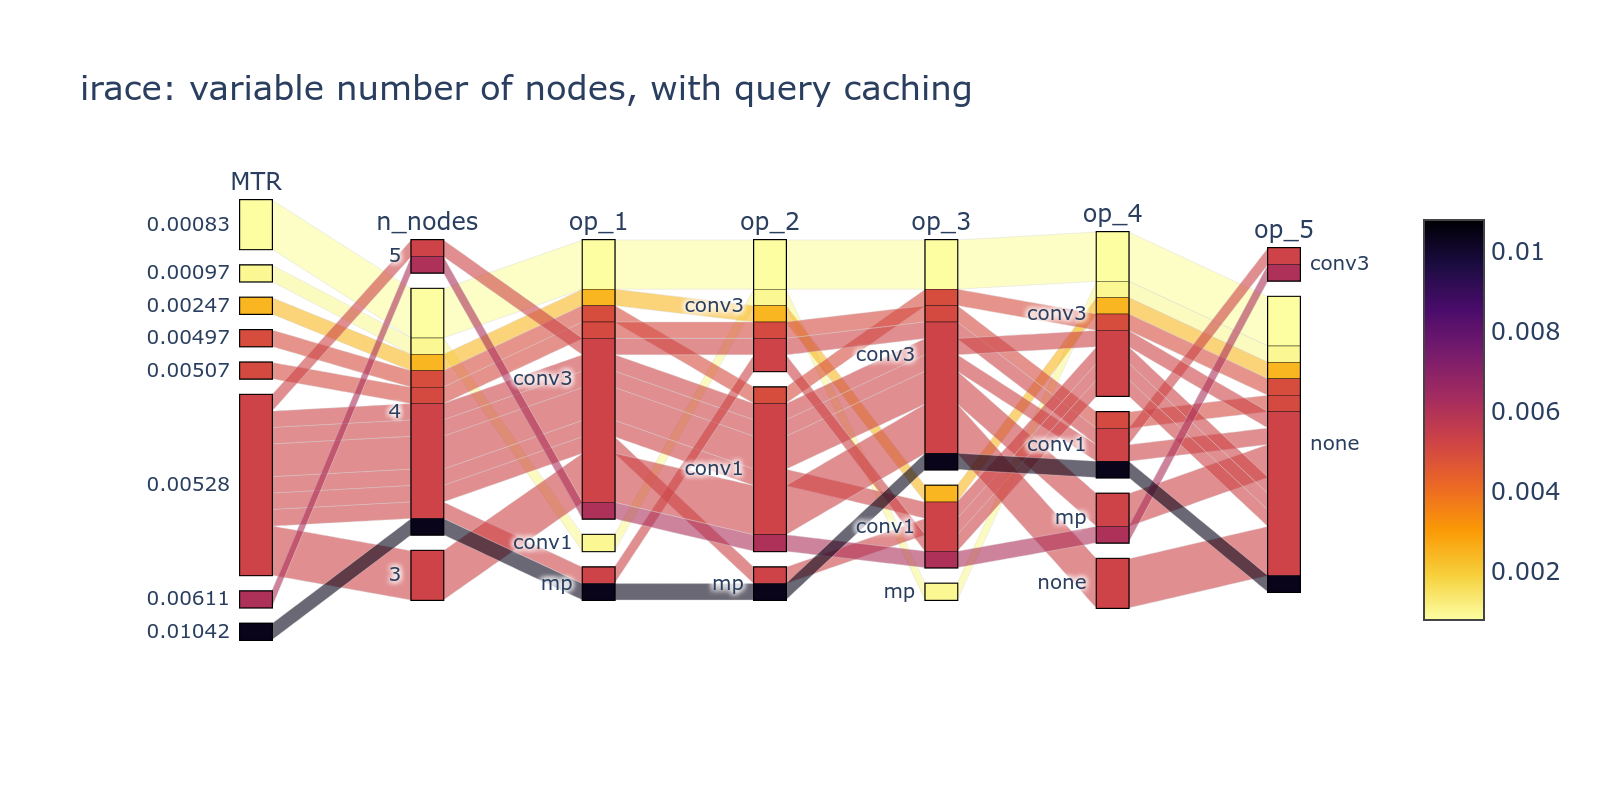
\includegraphics[width=0.47\linewidth, clip=true, trim=140px 150px 40px 150px]{imgs/parcat/irace-vnn.png}
% \caption{Parallel categories plots of the 20 architectures selected by SMAC (top) RE (middle) and \irace (bottom) with variable number of nodes, no caching (left), caching (right).}
% \label{fig:cv-co}
% \end{figure*}

% %!TEX root = ../emo.tex
\section{Conclusion}
\label{sec:conclusion}

Deep learning breakthroughs in challenging fields such as computer vision have redefined the research in neural architecture search~(NAS~\cite{ReaAggHuaLe2019re,ZopLe2017nas,ZopVasShlLeh2018scalable}). Besides the traditional contributions from neuroevolution, other effective algorithm classes have shown interesting results, such as algorithm configuration~(AC~\cite{ElsMetHut2019nas-survey}). However, the characteristics of deep learning scenarios differ considerably from optimization scenarios for which most effective ACs have been devised. In addition, the computational cost incurred for evaluating architectures currently prohibits extensive ACs runs.

\nasbench is a first effort towards comparability of NAS algorithms. Besides reusable data, authors also provide relevant guidelines for the evaluation and proposal of algorithms. In this work, we have proposed different ways in which the insights produced from this benchmark can be enriched, the most significant being the bi-objective formulation that enables an anytime performance assessment. Not surprisingly, the evaluation of \irace~\cite{LopDubPerStuBir2016irace}, RE~\cite{ReaAggHuaLe2019re}, and SMAC~\cite{HutHooLey2011lion} show that the relative performance of the techniques is not always the same from a final-quality or an anytime performance perspective.

A second contribution from our work is to study the effects of design choices embedded in the original \nasbench assessment. Specifically, we discuss the effects of a variable-sized encoding and caching, and demonstrate that algorithms are affected in different ways by these alternative setups. Finally, we argue against the use of an excessive number of algorithm repetitions, providing evidence that the budget of a configurator could be better spent on more instances or evaluating more architectures.

Besides the future work possibilities discussed along the paper, we highlight two other important pathways. The first is how to account for architecture training time besides accuracy, likely in a bi-objective formulation of architecture evaluation. The second is extending \nasbench to account for more datasets, so effective algorithms devised for multi-instance configuration may identify architectures that are high-performing across different datasets. Altogether, the benefits of these investigations may contribute to reduce dataset-dependent, computationally prohibitive campaigns.

% \section*{Acknowledgment}
% Leslie P\'erez C\'aceres acknowledges the support of Fondecyt project \#11190135.

\appendices
\section{Benchmarking \irace hyperparameters}
Given that \irace has not being applied to tackle \nasbench, we study its performance with different setups for a fair comparison with the other \nasbench techniques. We note that when dealing with known benchmarks, ACs can benefit from tailored setups as they can exploit known characteristics of the benchmarks.

% \leslie{}{NOTE: I would suggest to omit the experiments with fixed number of configurations and also the ones that set the configuration budget as number of experiments, as they are not the best performing and it might simplify the analysis.}

We performed 20 repetitions of \irace setting 10 million TPU seconds as total configuration budget and evaluate the performance obtained by the following setup options:

\begin{description}[style=unboxed, leftmargin=0px]
\item[Estimation budget] Budget assigned for the initial estimation of the average execution time of an evaluation. We perform experiments with 2\% and 0.2\% of the total configuration time for budget estimation.
\item[First test] Number of evaluations required to perform the first elimination test in a race. We perform experiments with 2 and 3 evaluations for applying the initial test.
\end{description}

For further details of these setup options we refer to~\cite{LopDubPerStuBir2016irace}. Figure~\ref{fig:irace-setup-performance} gives the ECDFs of the final quality obtained by the different setups of \irace. The best overall performance is obtained by setting the estimation budget to $2\%$ of the total configuration time and allowing 3 evaluations before the first elimination test (mean test regret $0.002837$).
\begin{figure*}
	\centering
	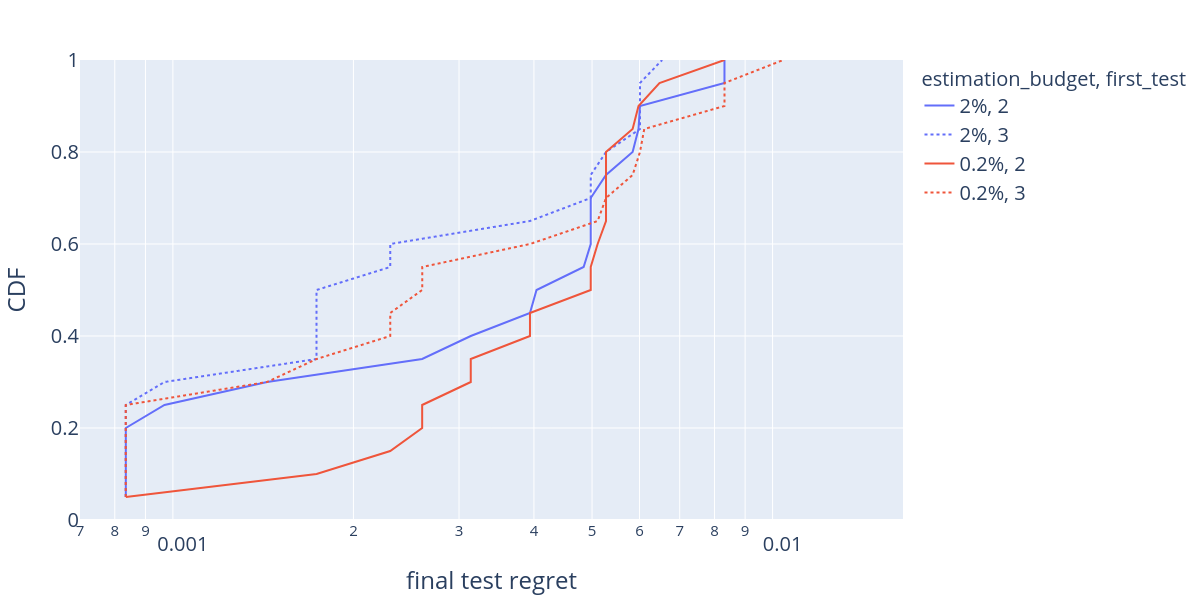
\includegraphics[width=0.75\textwidth]{imgs/irace-setup-ecdf.png}
	\caption{Empirical cumulative distribution function~($x$-axis) of the final regret~($y$-axis) from 20 runs of each \irace setup.}
	\label{fig:irace-setup-performance}
\end{figure*}

\section{High-performing configurations plots}
Here we present parallel categories plots representing the architectures selected by the different NAS techniques. Figure~\ref{fig:pc-fnn} shows the configurations selected when using a fixed number of nodes, while Figure~\ref{fig:pc-vnn} shows those using a variable number of nodes. As in the paper, only NAS hyperpameters related to the node label list are given~(\textit{op$_1$}-\textit{op$_5$}), corresponding to each vertex of the DAG model, i.e. each layer of the selected neural network, for legibility's sake. Furthermore, color scaling (on the same range for all plots) reflects the mean test regret, also depicted as a discretized variable in the left-most column of the plots. Do note that, since topology is defined by the adjacency matrix, no layer order or architecture size should be assumed.

\begin{figure*}
\centering
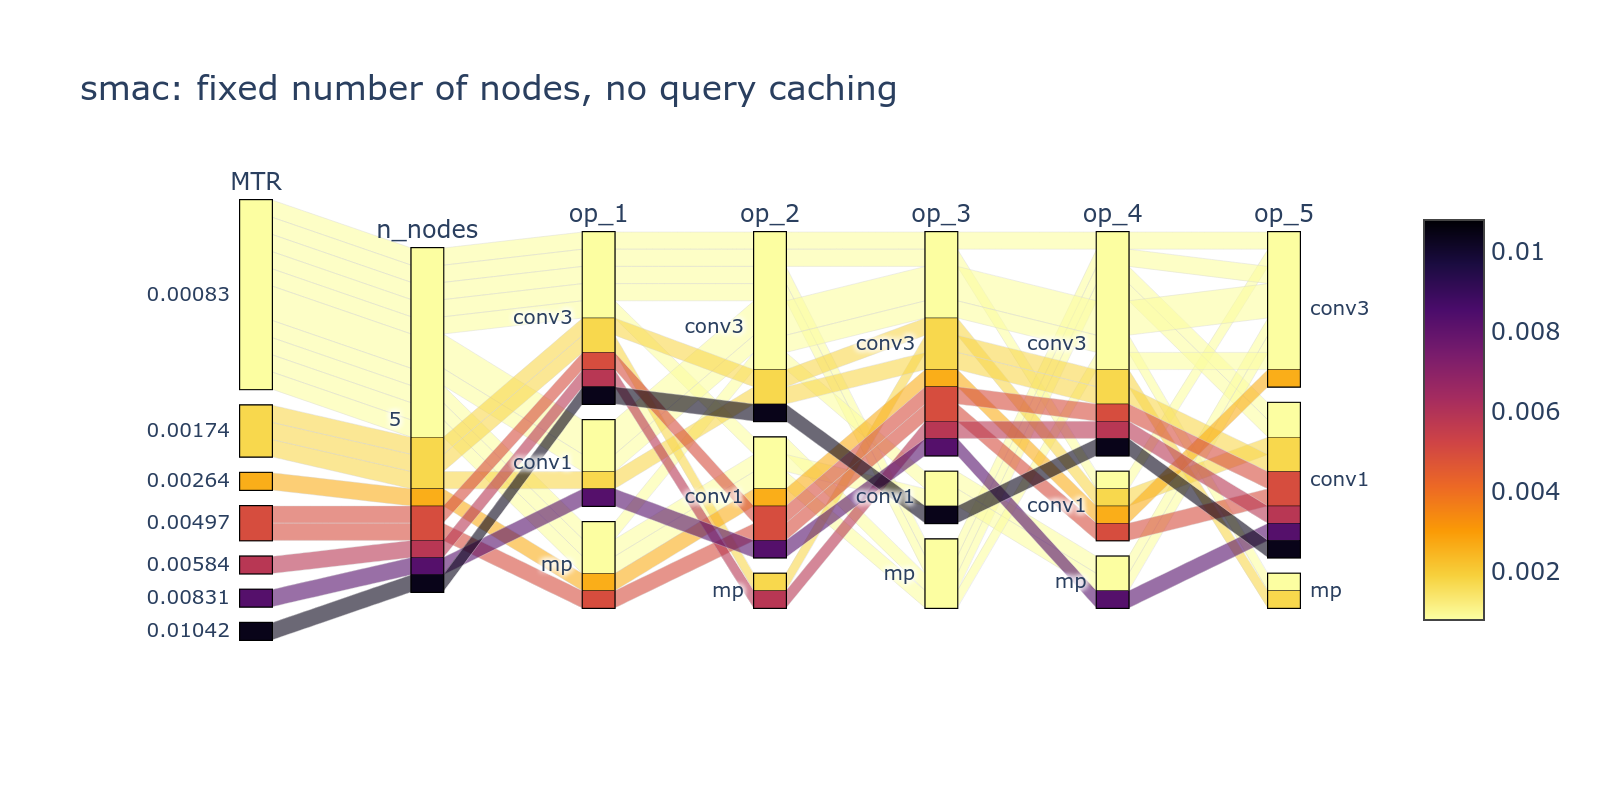
\includegraphics[width=0.47\linewidth, clip=true, trim=140px 150px 40px 150px]{imgs/parcat/smac-fnn-nc.png}
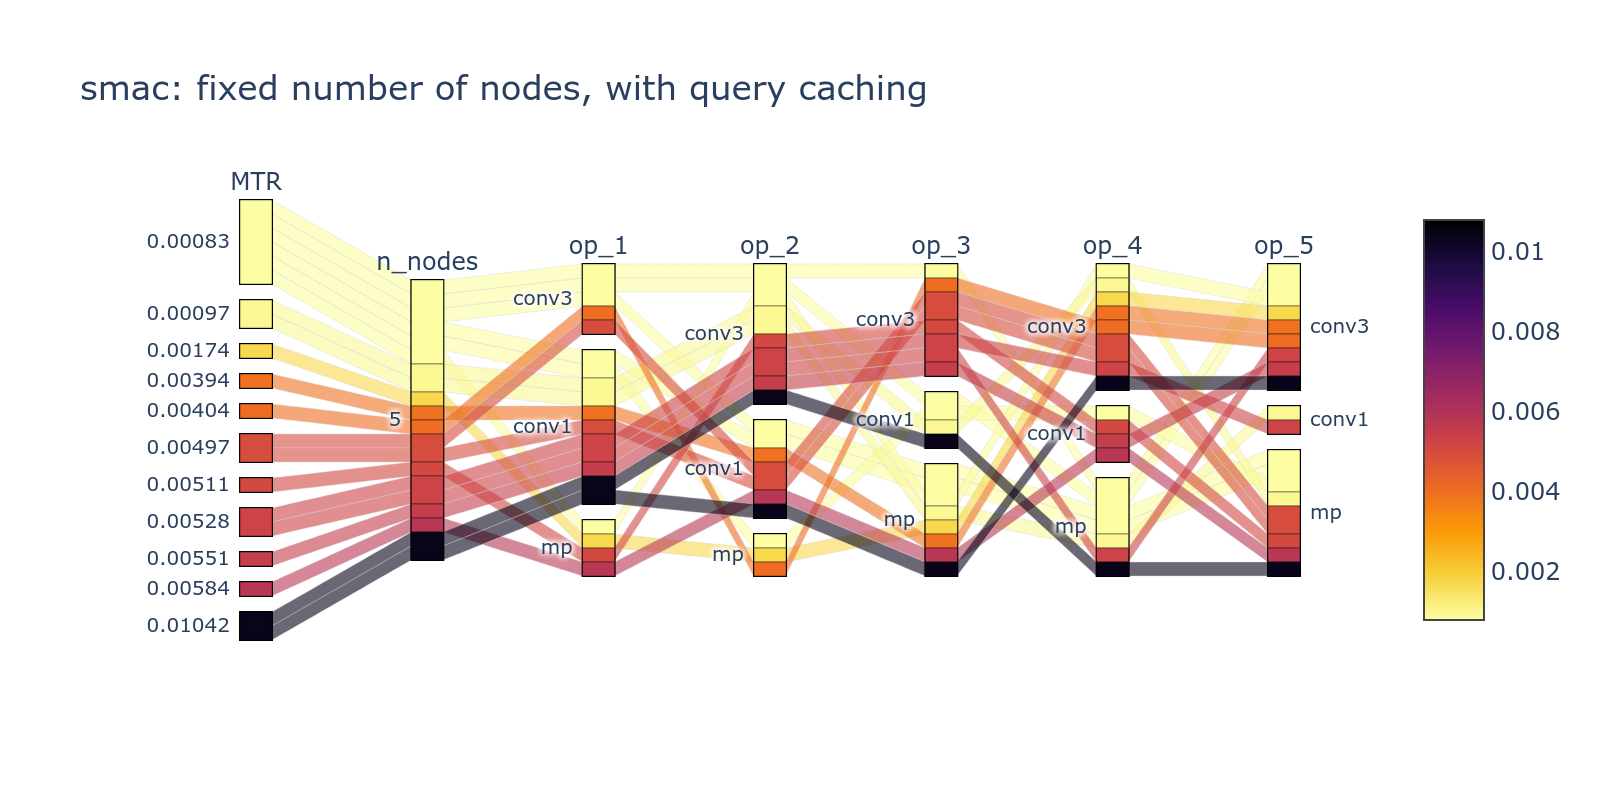
\includegraphics[width=0.47\linewidth, clip=true, trim=140px 150px 40px 150px]{imgs/parcat/smac-fnn.png}
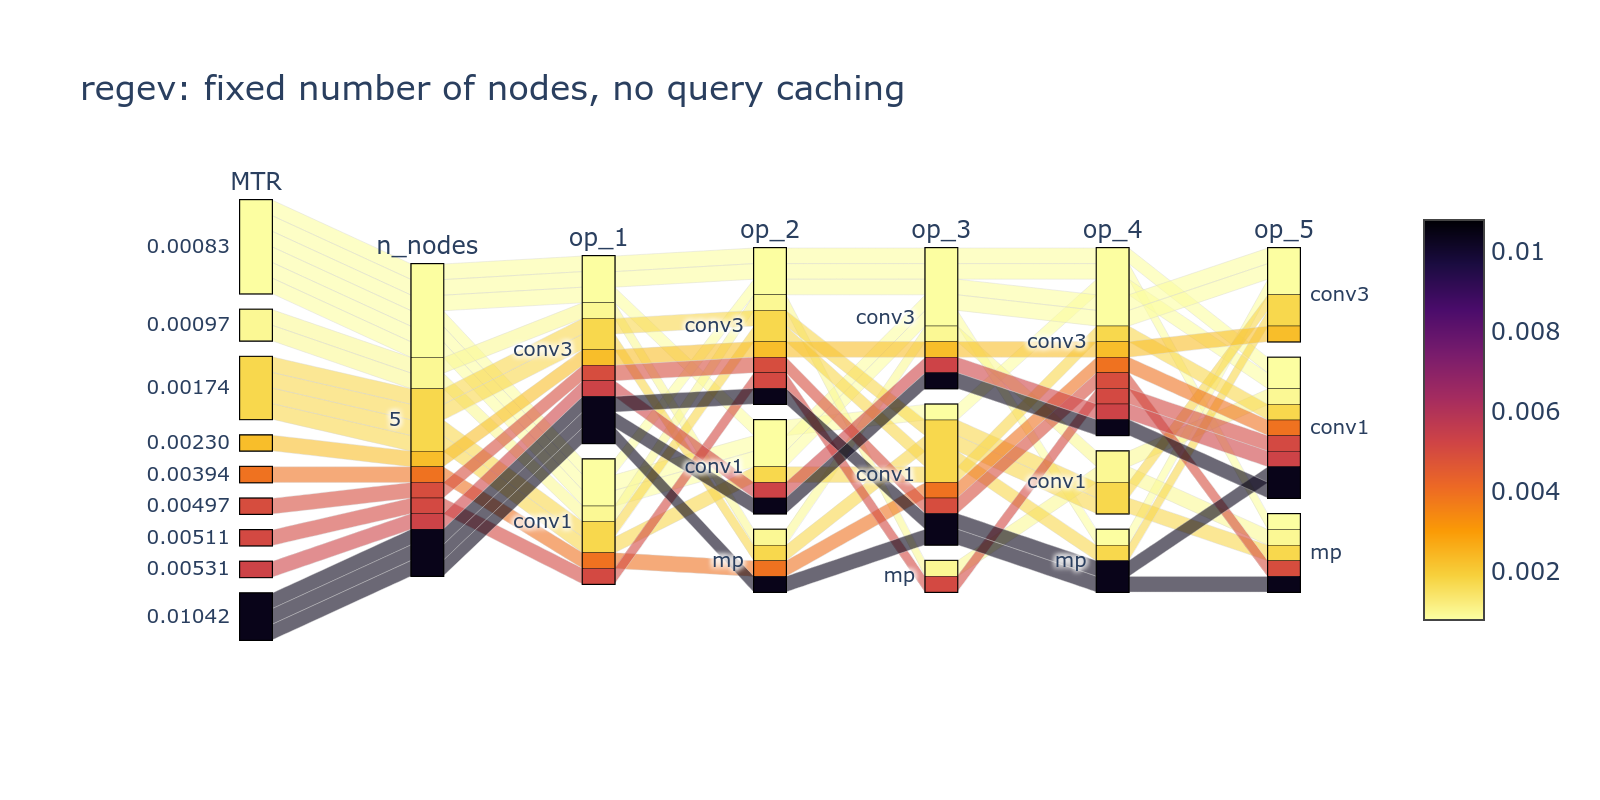
\includegraphics[width=0.47\linewidth, clip=true, trim=140px 150px 40px 150px]{imgs/parcat/re-fnn-nc.png}
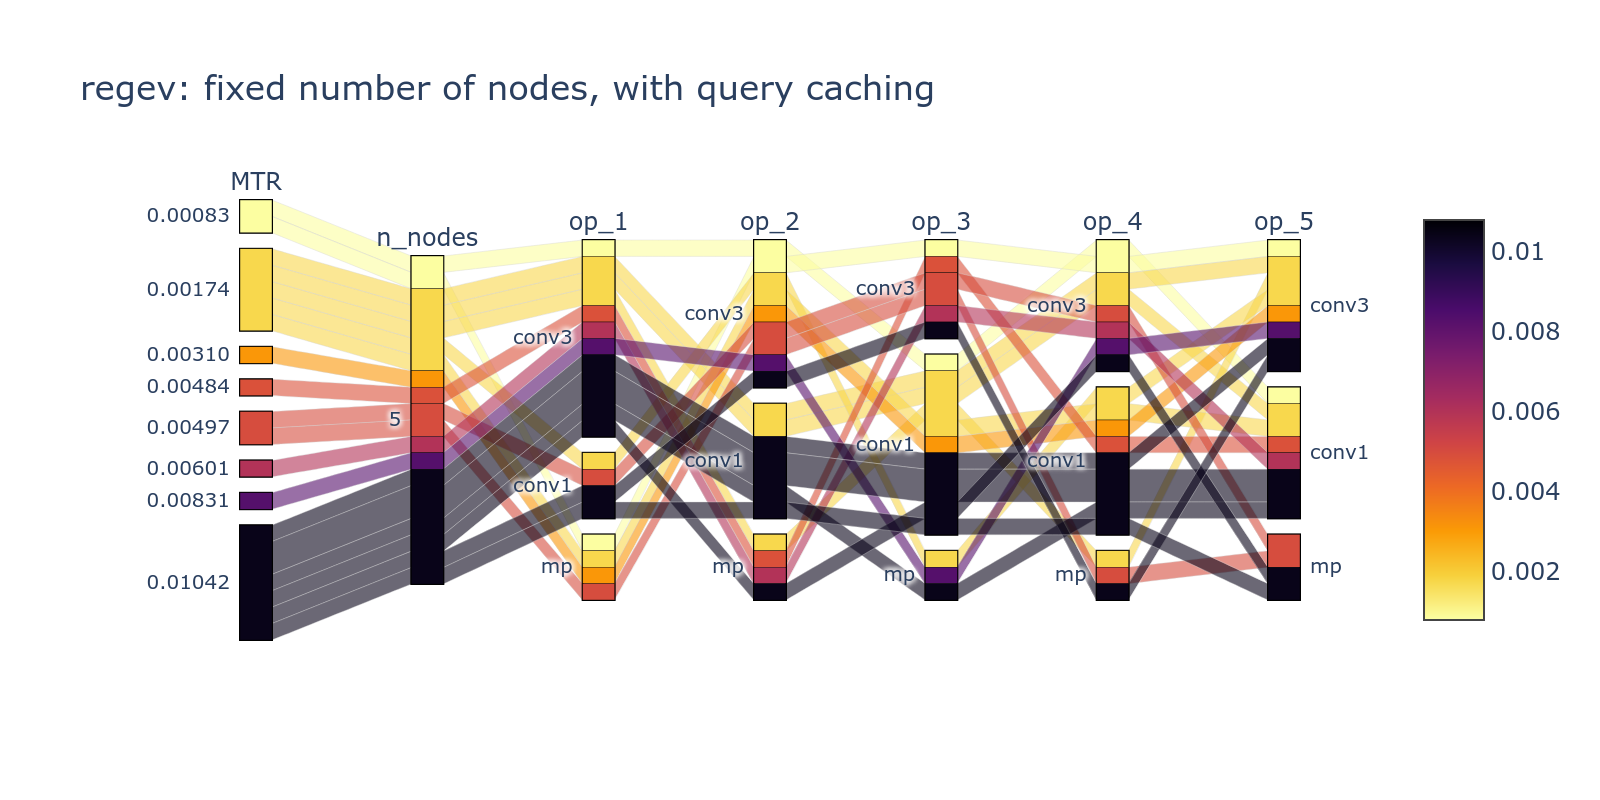
\includegraphics[width=0.47\linewidth, clip=true, trim=140px 150px 40px 150px]{imgs/parcat/re-fnn.png}
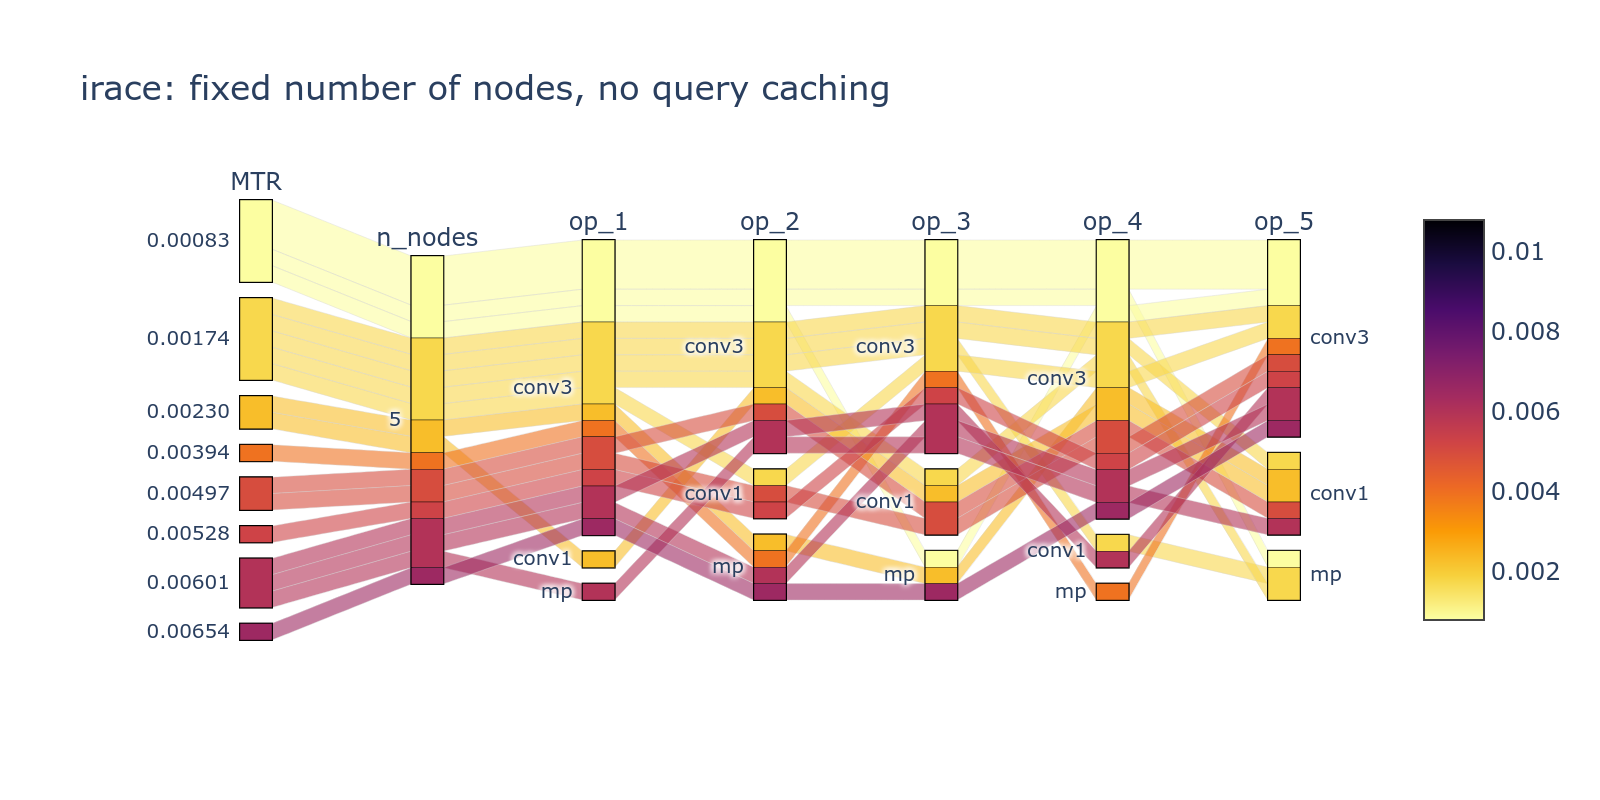
\includegraphics[width=0.47\linewidth, clip=true, trim=140px 150px 40px 150px]{imgs/parcat/irace-fnn-nc.png}
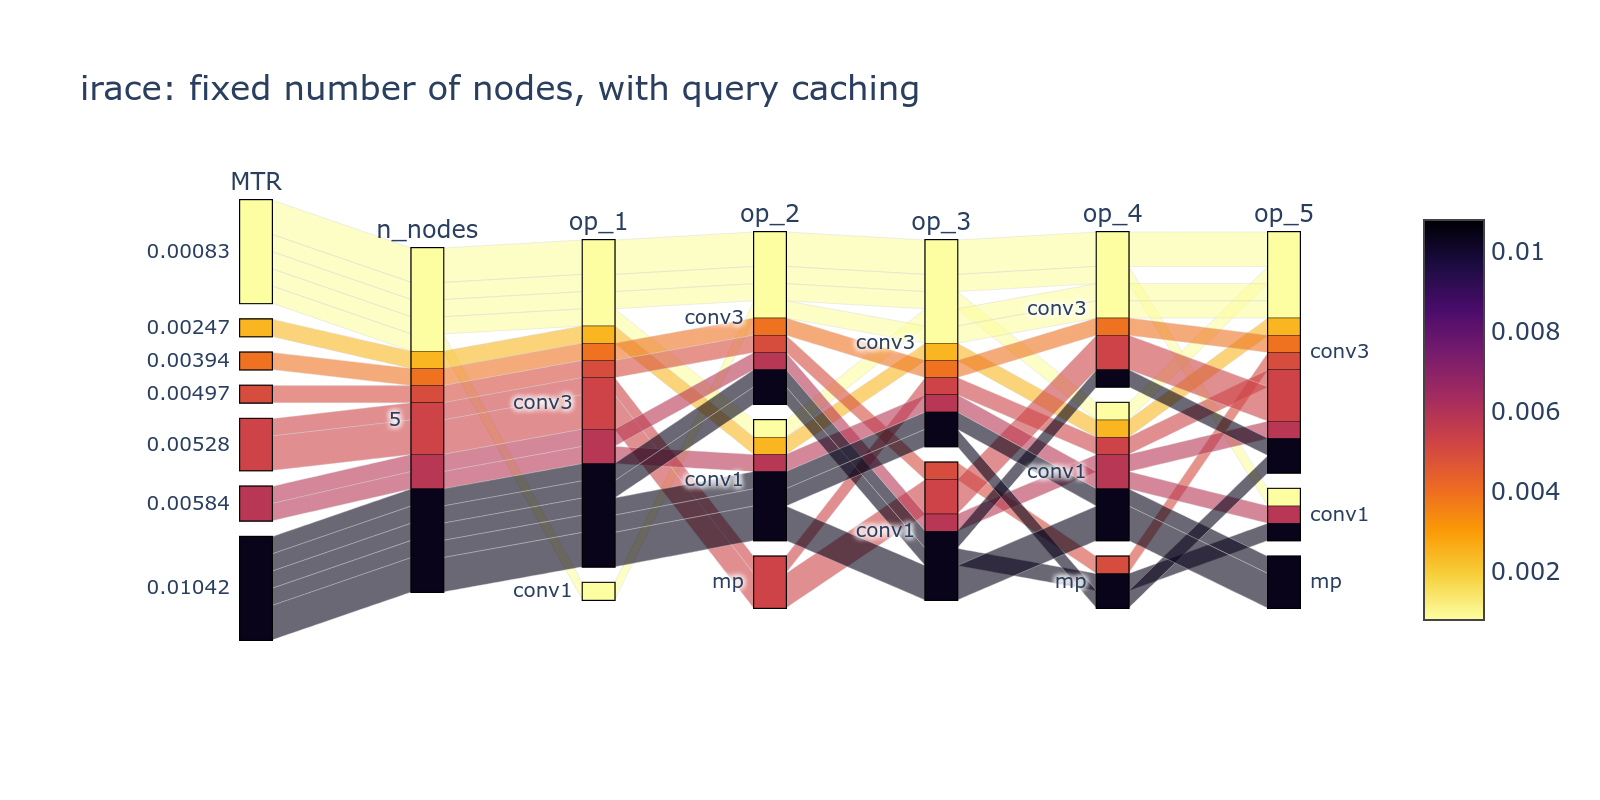
\includegraphics[width=0.47\linewidth, clip=true, trim=140px 150px 40px 150px]{imgs/parcat/irace-fnn.png}
\caption{Parallel categories plots of the 20 architectures selected by SMAC (top), RE (middle), and \irace (bottom) with fixed number of nodes, no caching (left), caching (right).}
\label{fig:pc-fnn}
\end{figure*}


\begin{figure*}
\centering
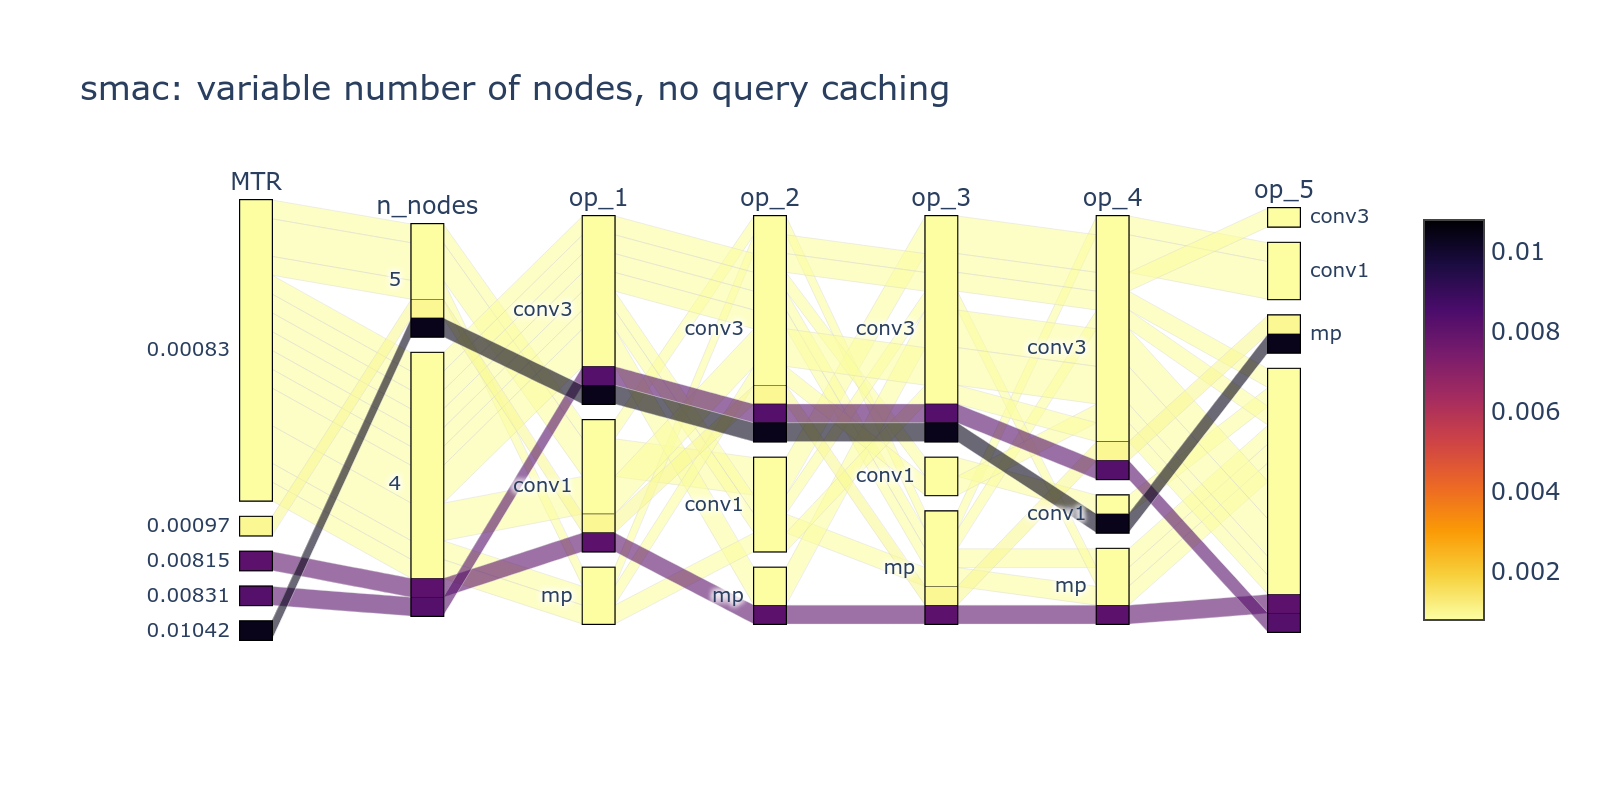
\includegraphics[width=0.47\linewidth, clip=true, trim=140px 150px 40px 150px]{imgs/parcat/smac-vnn-nc.png}
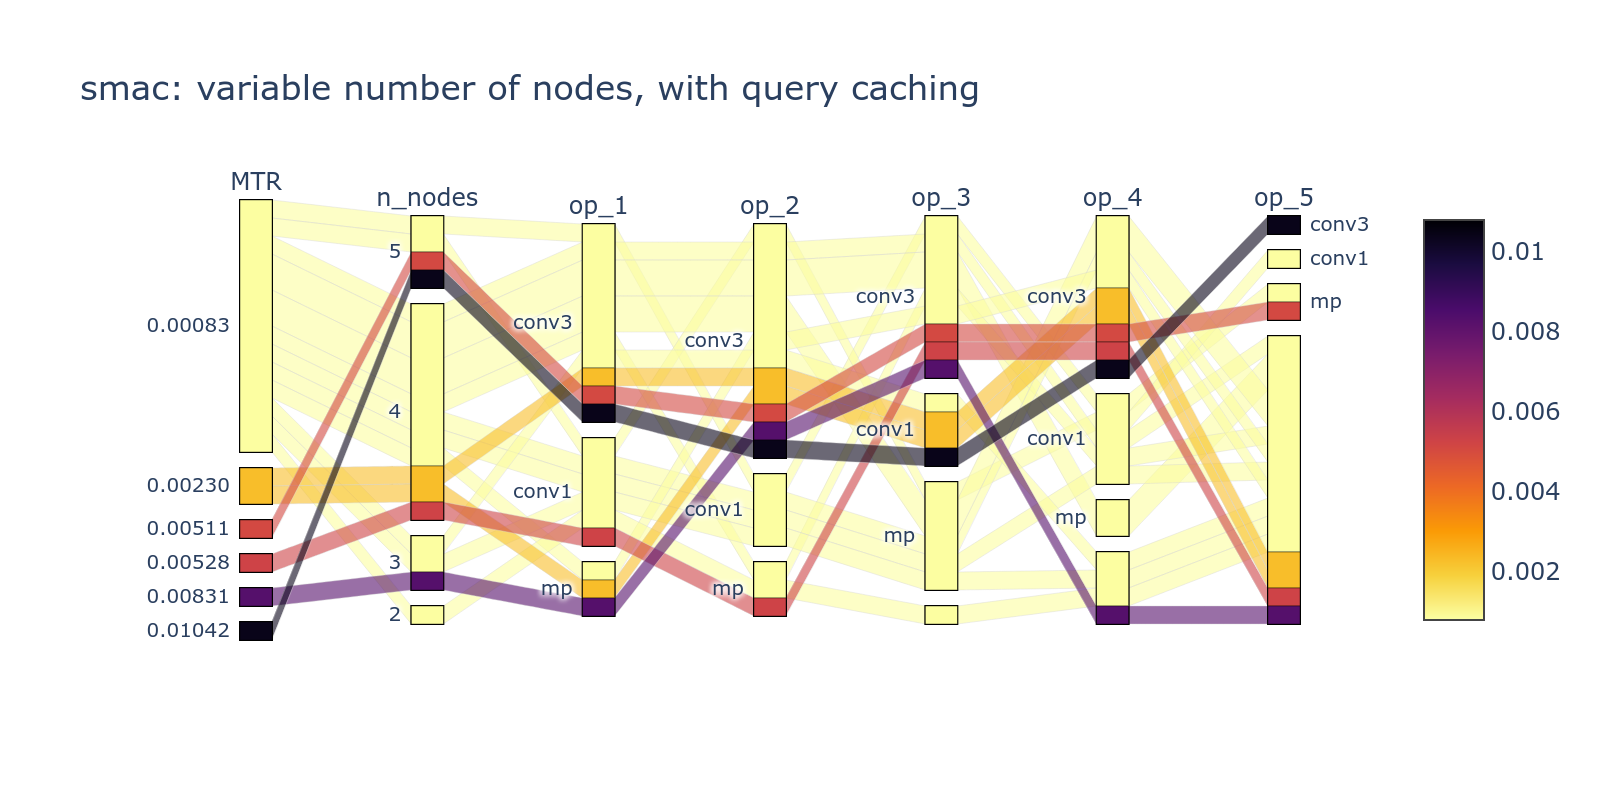
\includegraphics[width=0.47\linewidth, clip=true, trim=140px 150px 40px 150px]{imgs/parcat/smac-vnn.png}
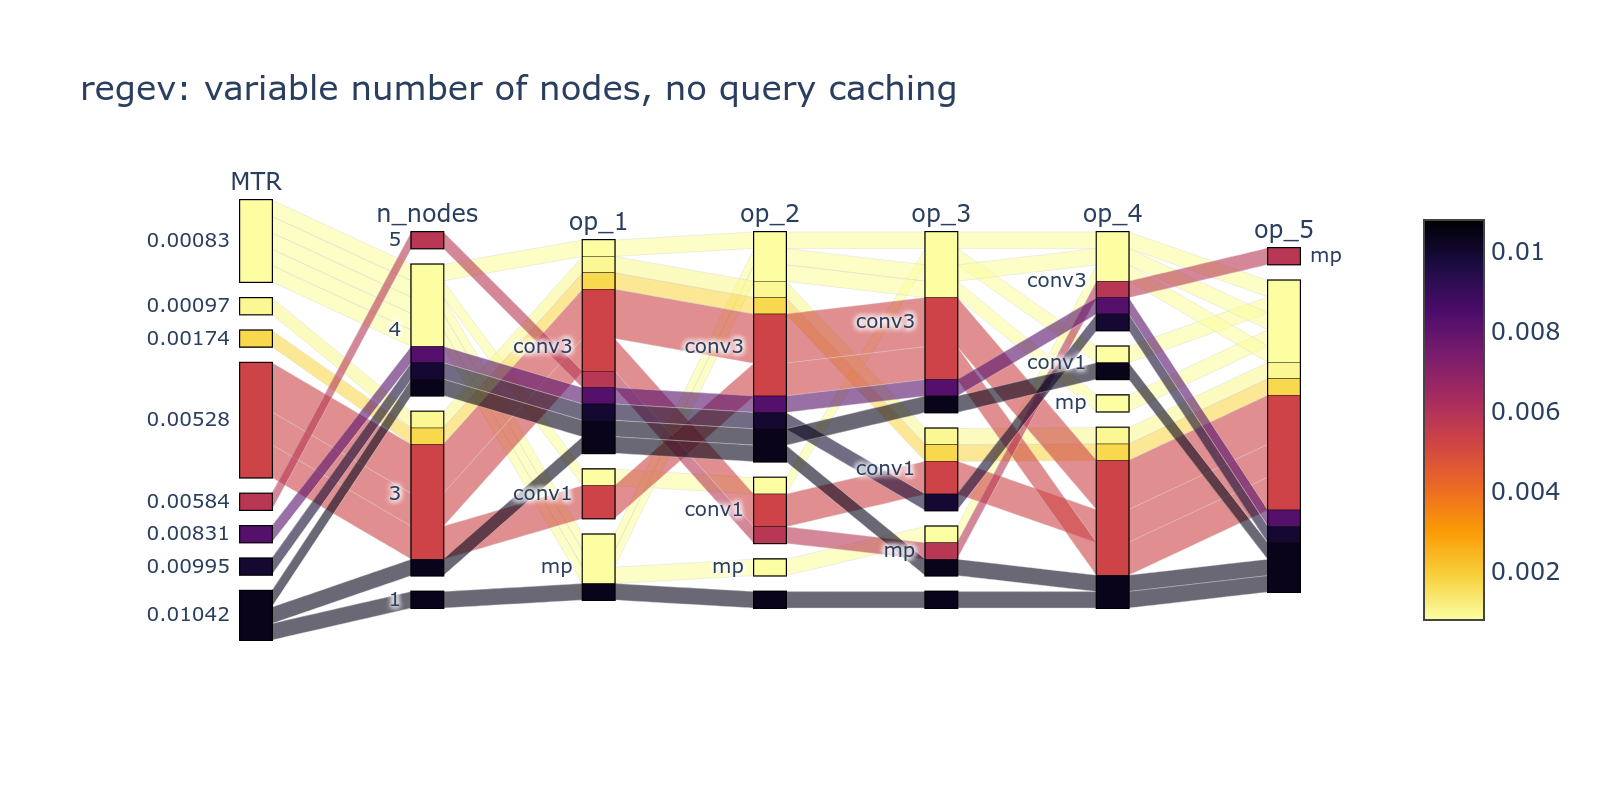
\includegraphics[width=0.47\linewidth, clip=true, trim=140px 150px 40px 150px]{imgs/parcat/re-vnn-nc.png}
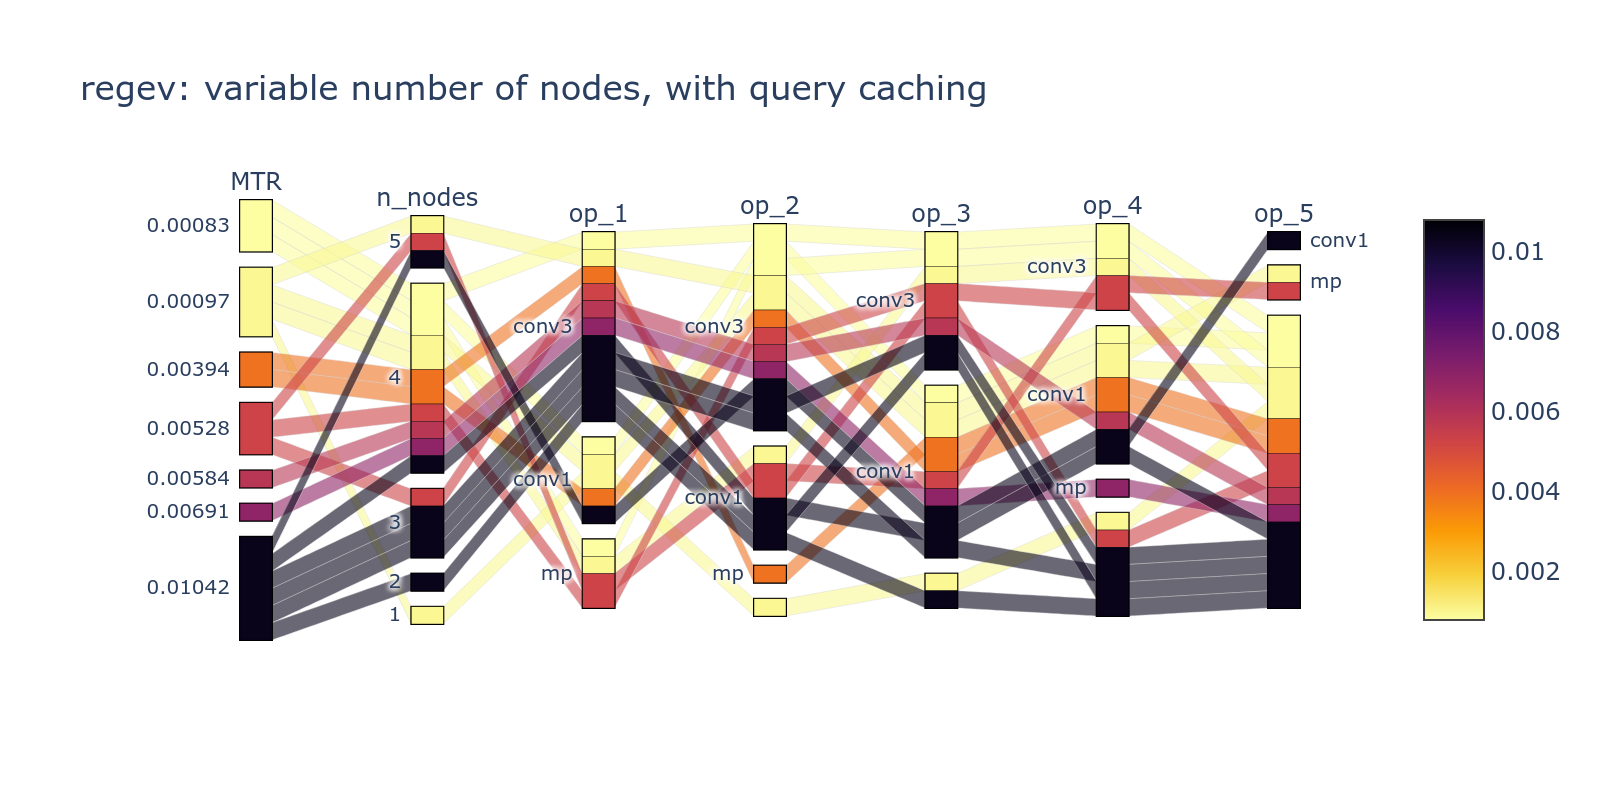
\includegraphics[width=0.47\linewidth, clip=true, trim=140px 150px 40px 150px]{imgs/parcat/re-vnn.png}
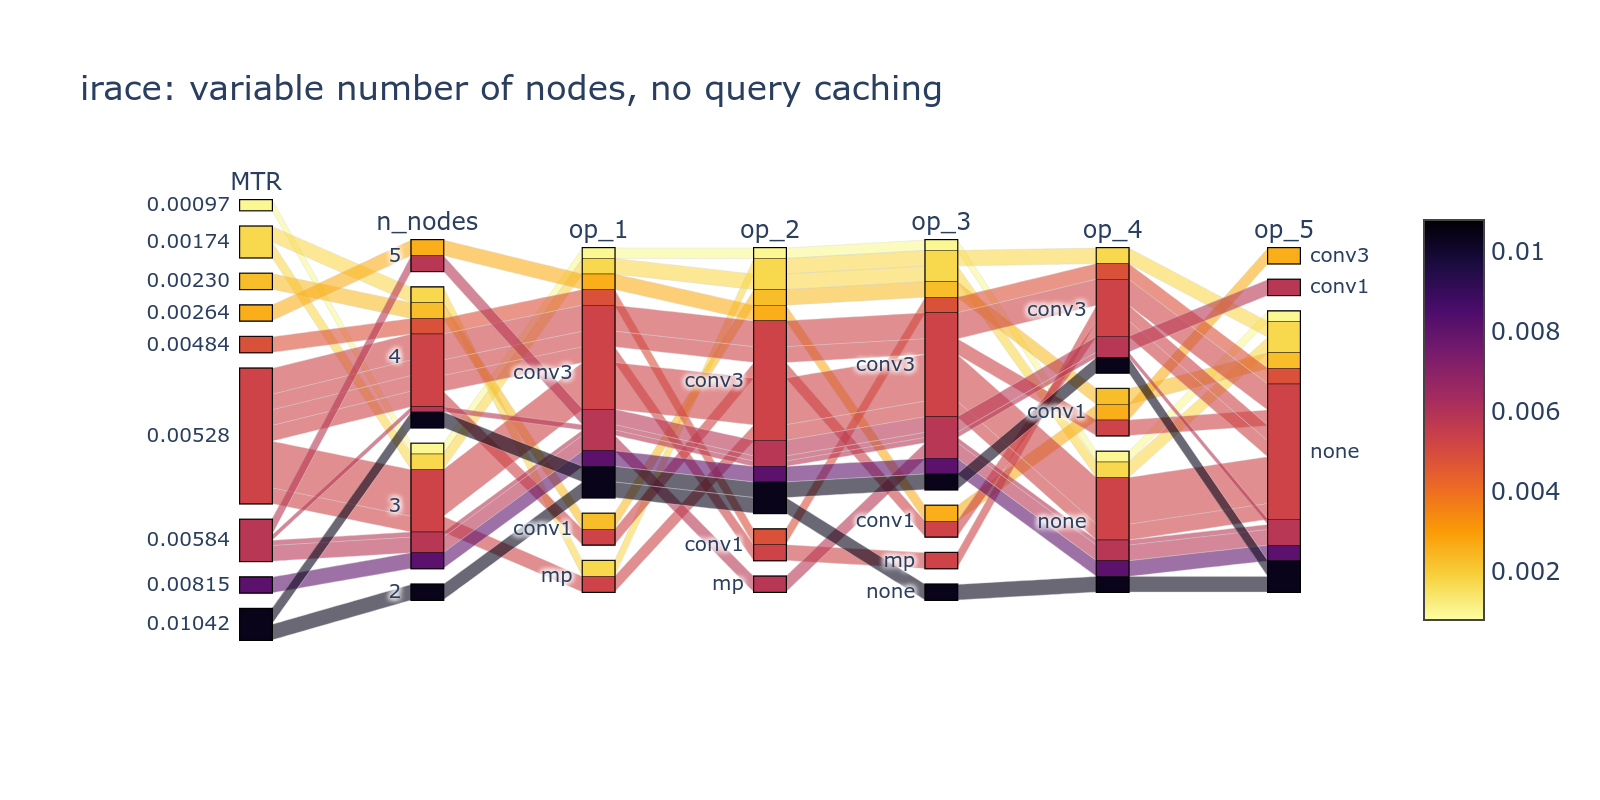
\includegraphics[width=0.47\linewidth, clip=true, trim=140px 150px 40px 150px]{imgs/parcat/irace-vnn-nc.png}
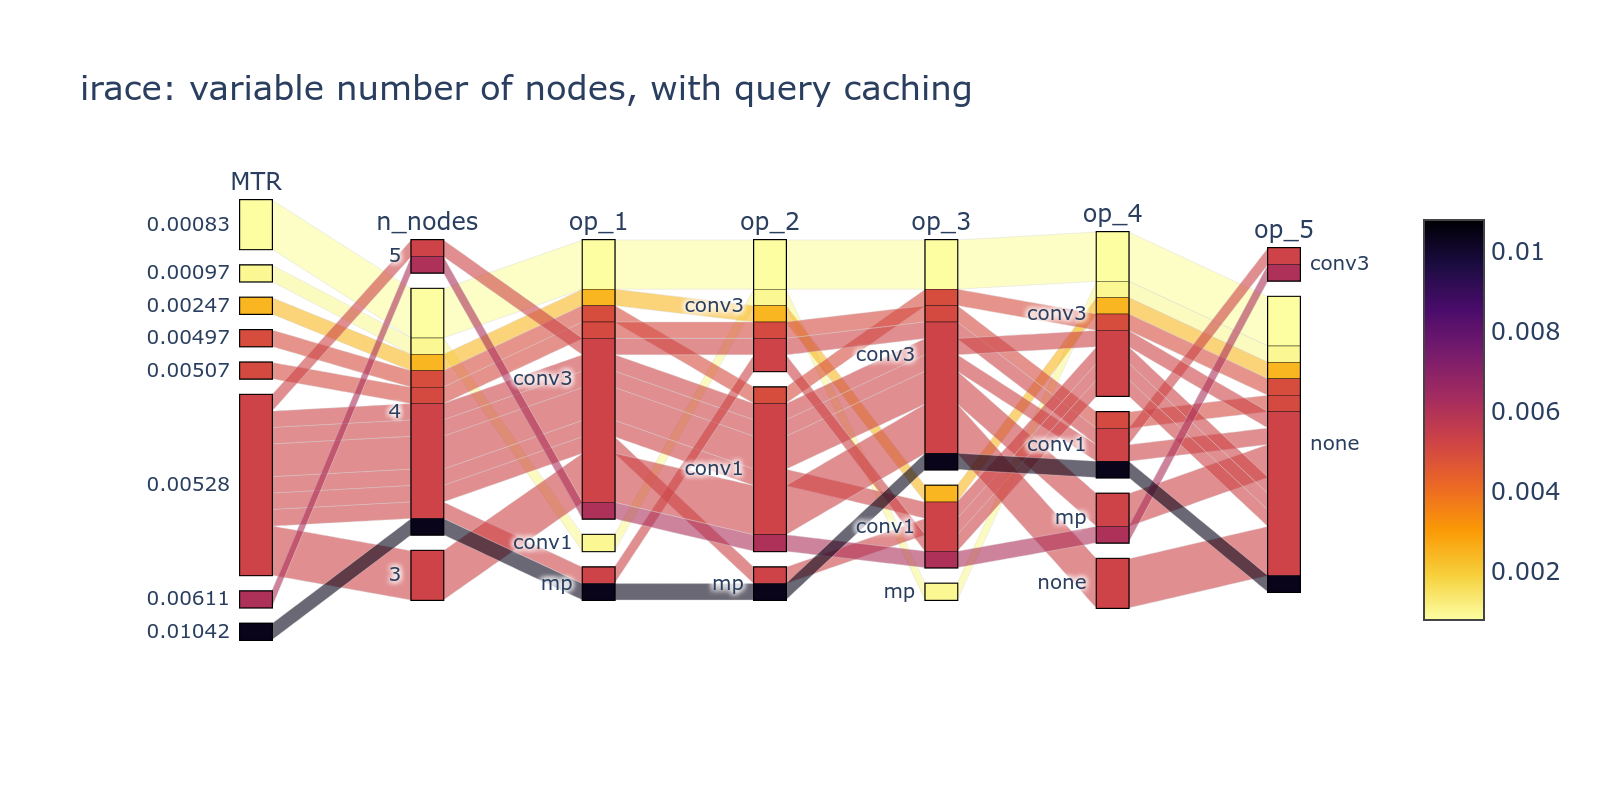
\includegraphics[width=0.47\linewidth, clip=true, trim=140px 150px 40px 150px]{imgs/parcat/irace-vnn.png}
\caption{Parallel categories plots of the 20 architectures selected by SMAC (top) RE (middle) and \irace (bottom) with variable number of nodes, no caching (left), caching (right).}
\label{fig:pc-vnn}
\end{figure*}

\section{Runtime statistics}
Here we give runtime (wallclock) statistics for all three algorithms in their different experimental setups in Figure~\ref{fig:wallclock-times}. Abbreviations for experimental setups are used as in the paper: O for original; VS for variable-sized; C for caching; and CVS for caching and variable-sized. Runtime along the $y$ axis is given in hours:minutes:seconds format.

% \begin{figure*}
% 	\centering

% 	\begin{subfigure}[t]{0.3\textwidth}
% 	\centering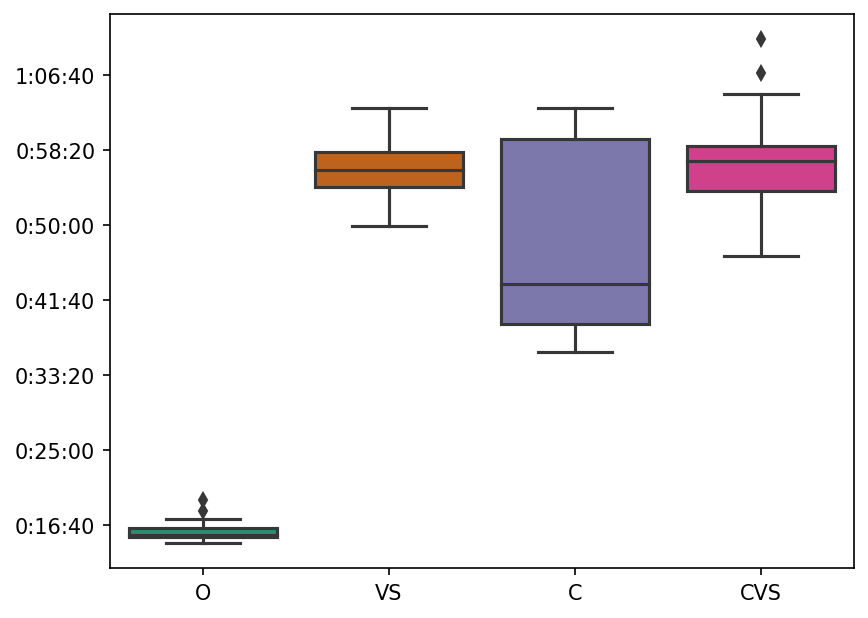
\includegraphics[width=\textwidth]{imgs/irace-times-boxplots.png}
% 	% \caption{\irace}
% 	\end{subfigure}
% 	\begin{subfigure}[t]{0.3\textwidth}
% 	\centering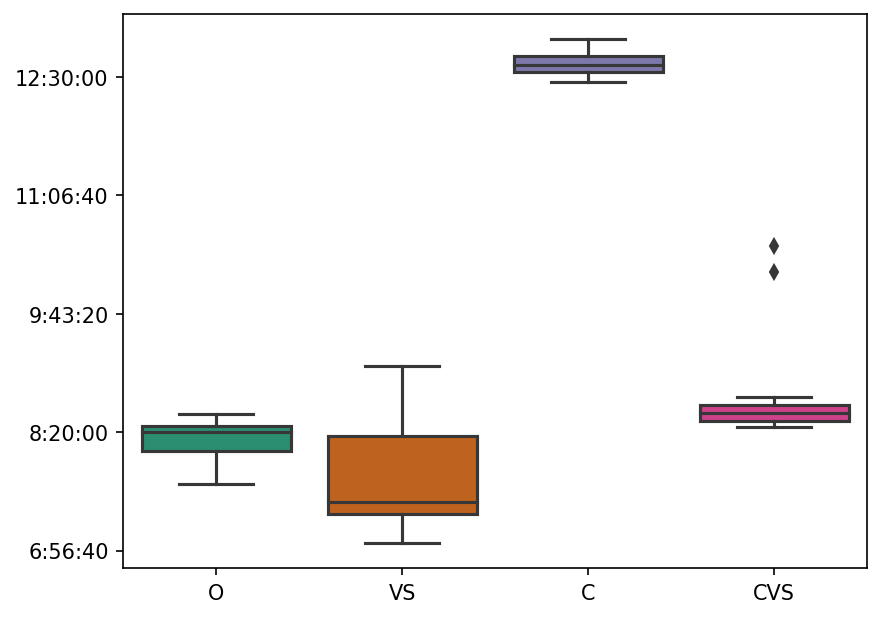
\includegraphics[width=\textwidth]{imgs/smac-times-boxplots.png}
% 	% \caption{SMAC}
% 	\end{subfigure}[t]{0.3\textwidth}
% 	\begin{subfigure}
% 	\centering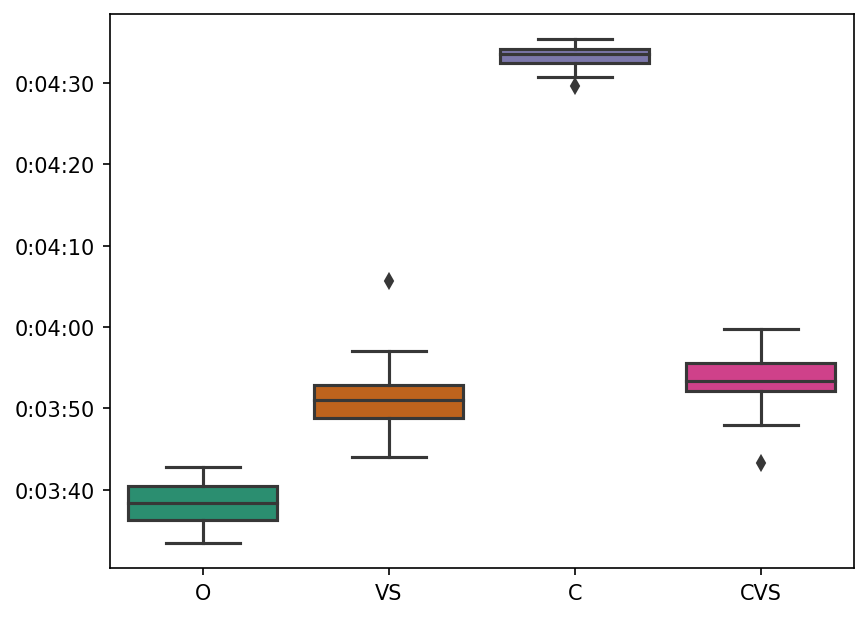
\includegraphics[width=\textwidth]{imgs/regev-times-boxplots.png}
% 	% \caption{RE}
% 	\end{subfigure}

% 	\caption{Boxplots representing wallclock runtimes (over 20 runs) of each algorithm under different experimental setups}
% 	\label{fig:wallclock-times}
% \end{figure*}

\begin{figure*}
\centerline{%
\subfigure[\irace]{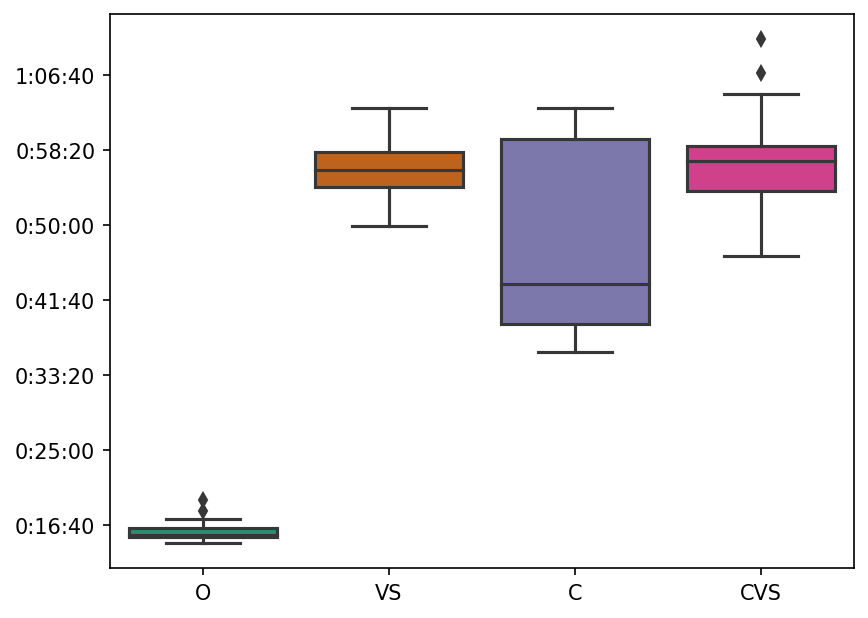
\includegraphics[width=0.3\textwidth]{imgs/irace-times-boxplots.png}}
\hfil
\subfigure[SMAC]{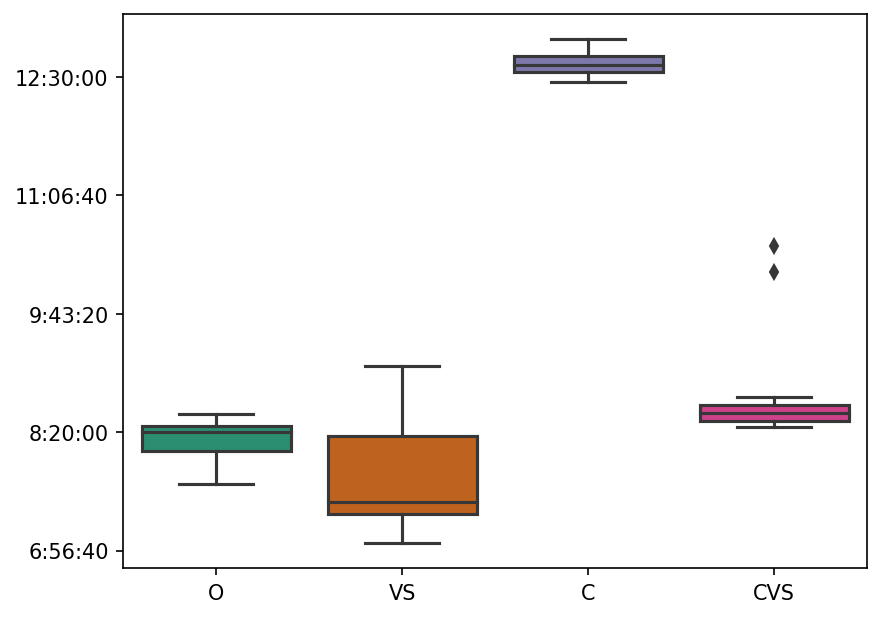
\includegraphics[width=0.3\textwidth]{imgs/smac-times-boxplots.png}}
\hfil
\subfigure[RE]{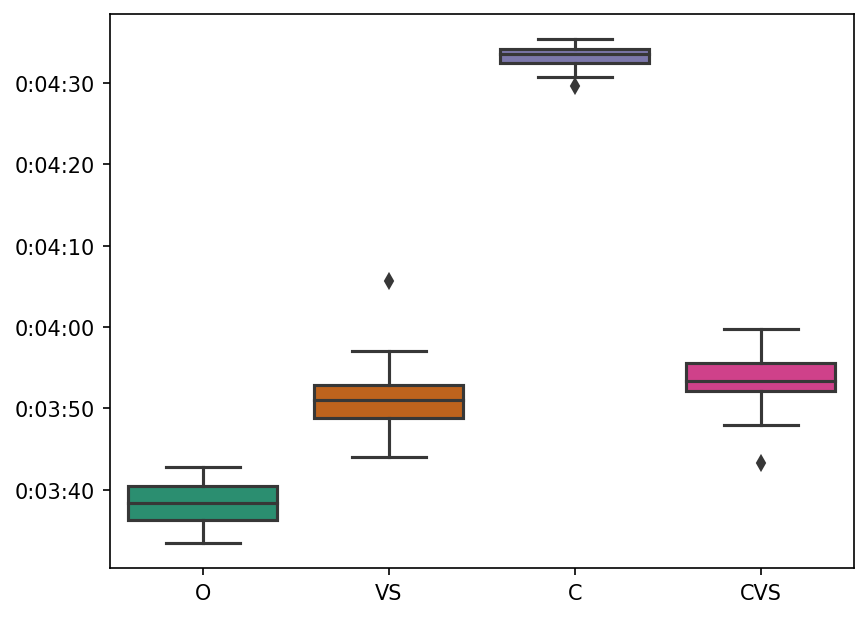
\includegraphics[width=0.3\textwidth]{imgs/regev-times-boxplots.png}}
}
\caption{Boxplots representing wallclock runtimes (over 20 runs) of each algorithm under different experimental setups}
\label{fig:wallclock-times}
\end{figure*}


\bibliographystyle{ieeetran}
\bibliography{main}

\end{document}
